%%%%%%%% ICML 2026 / FM4LS WORKSHOP CAMERA-READY %%%%%%%%%%%%%%%%%%%%%%%%%
% PerturbCausal: Virtual Cell Model Predictions Do Not Substitute
% for Real Perturb-seq in Causal Network Recovery
%
% Camera-ready for the FM4LS workshop @ ICML 2026.
%   - Main content (title through Conclusion, before \appendix) <= 5 pages.
%   - References and appendix are unlimited and excluded from the page count;
%     overflow from the original full manuscript has been relocated into the
%     appendix VERBATIM (no number, CI, p-value, table value, or citation
%     key was changed).
%   - icml2026 style is set to [accepted] for non-anonymous camera-ready.
%
% To compile (drop icml2026.sty into the same directory):
%   pdflatex CausalCellBench_FM4LS_CameraReady.tex
%   bibtex   CausalCellBench_FM4LS_CameraReady   (uses thebibliography, so
%            bibtex is not strictly required; run pdflatex x3 for cross-refs)
%   pdflatex CausalCellBench_FM4LS_CameraReady.tex
%   pdflatex CausalCellBench_FM4LS_CameraReady.tex

\documentclass{article}

% Recommended, but optional, packages for figures and better typesetting
\usepackage{microtype}
\usepackage{graphicx}
\usepackage{subcaption}
\usepackage{booktabs} % for professional tables
\usepackage{multirow}
\usepackage{enumitem} % for enumerate options in appendix
\usepackage{amsmath, amssymb, amsthm}
\usepackage{xcolor}
\usepackage{url}

% hyperref makes hyperlinks in the resulting PDF.
% If your build breaks (sometimes hyperref breaks), please remove
% the package and try again.
\usepackage[colorlinks=true,
            linkcolor=blue,
            citecolor=blue,
            urlcolor=blue]{hyperref}

% FM4LS @ ICML 2026 --- camera-ready (non-anonymous). Use the [accepted]
% option of the icml2026 style file to reveal authorship.
\usepackage[accepted]{icml2026}

% For theorems and such
\usepackage{amsmath}
\usepackage{amssymb}
\usepackage{mathtools}
\usepackage{amsthm}

% if you use cleveref..
\usepackage[capitalize,noabbrev]{cleveref}

%%%%%%%%%%%%%%%%%%%%%%%%%%%%%%%%%%%%%%%%%%%%%%%%%%%%%%%%%%%%%%%%%%%%%%%%
%%% THEOREMS
\theoremstyle{plain}
\newtheorem{theorem}{Theorem}[section]
\newtheorem{proposition}[theorem]{Proposition}
\newtheorem{lemma}[theorem]{Lemma}
\newtheorem{corollary}[theorem]{Corollary}
\theoremstyle{definition}
\newtheorem{definition}[theorem]{Definition}
\newtheorem{assumption}[theorem]{Assumption}
\theoremstyle{remark}
\newtheorem{remark}[theorem]{Remark}

% The \icmltitle running for the citations / page header
\icmltitlerunning{VCMs Do Not Substitute for Real Perturb-seq in Causal Recovery}

\begin{document}

\twocolumn[
\icmltitle{PerturbCausal: Virtual Cell Model Predictions Do Not Substitute \\
           for Real Perturb-seq in Causal Network Recovery}

\icmlsetsymbol{equal}{*}

\begin{icmlauthorlist}
\icmlauthor{Aayan Alwani}{ind}
\end{icmlauthorlist}

\icmlaffiliation{ind}{Independent Researcher}

\icmlcorrespondingauthor{Aayan Alwani}{alwaniaayan6@gmail.com}

% You may provide any keywords that you find helpful for describing your paper; these are used to populate
% the "keywords" metadata in the PDF but will not be shown in the document
\icmlkeywords{Virtual Cell Models, Causal Discovery, Perturb-seq, Gene Regulatory Networks, Calibration}

\vskip 0.3in
]

% this must go after the closing bracket ] following \twocolumn[ ...

% This command actually creates the footnote in the first column
% listing the affiliations and the copyright notice.
\printAffiliationsAndNotice{} % leave blank if no need to mention equal contribution

\begin{abstract}
Virtual cell models (VCMs) predict transcriptional responses to genetic perturbations and are promoted as in silico substitutes for CRISPR screens; \citet{ahlmanneltze2025} showed they fail to beat simple linear baselines at per-gene prediction. We ask whether predicted Perturb-seq can substitute for real Perturb-seq one step downstream, in causal network recovery. PerturbCausal holds the causal-discovery algorithm fixed and varies only the data source, scoring the network recovered from VCM predictions against the one the same algorithm recovers from real data. Evaluating four VCMs (GEARS, CPA, Geneformer, the 2025 Arc Institute STATE model) through four backends (GIES, inspre, PC, NOTEARS) on three datasets (K562, RPE1; CRISPRi, CRISPRa), no deep VCM exceeds a sparse linear ElasticNet comparator and none reaches real-data quality; STATE's single-seed advantage does not replicate. The failure has one signature: predicted effect-size distributions are inflated and nearly identical across perturbations, the pooled counterpart of mode collapse. Quantile-matching calibration corrects the magnitude marginal exactly yet leaves the causal gap open, locating the residual in joint structure that distributional calibration provably cannot reach. The benchmark and code are released as an open-source package.
\end{abstract}

%%%%%%%%%%%%%%%%%%%%%%%%%%%%%%%%%%%%%%%%%%%%%%%%%%%%%%%%%%%%%%%%%%%%%%%%
\section{Introduction}
\label{sec:intro}

Virtual cell models (VCMs) predict cellular responses to genetic perturbations and are proposed as substitutes for CRISPR screens that cost millions of dollars per cell line~\citep{replogle2022,bunne2024}. The dominant evaluation paradigm---PerturBench~\citep{wu2024perturbench}, the Virtual Cell Challenge~\citep{roohani2025vcc}, and the Ahlmann-Eltze \& Huber comparison~\citep{ahlmanneltze2025}---measures per-gene reconstruction accuracy, where graph neural networks (GEARS;~\citealt{roohani2024gears}), conditional VAEs (CPA;~\citealt{lotfollahi2023cpa}), and foundation transformers (Geneformer, scGPT;~\citealt{theodoris2023geneformer,cui2024scgpt}) consistently fail to beat simple linear baselines.

Reconstruction accuracy is a property of the marginal distribution of effects. The downstream applications that motivate VCMs---combination prediction, drug target identification, and gene regulatory network (GRN) inference---depend instead on the joint distribution across genes~\citep{chevalley2025causalbench,vc_causal_2025}: a model can match every per-gene mean and still distort the gene-gene covariance and conditional-independence structure that interventional causal discovery exploits. CausalBench runs causal discovery on real Perturb-seq~\citep{chevalley2025causalbench} but does not test whether VCM predictions can substitute for that real data; a NeurIPS 2025 perspective called for such an evaluation without implementing one~\citep{vc_causal_2025}. Adjacent work surfaced the pieces---mode collapse in perturbation models~\citep{mejia2025diversity}, poorly calibrated prediction metrics~\citep{miller2025calibrated}, and inspre for large-scale causal discovery from interventional data~\citep{brown2025inspre}---but none integrates VCM predictions into a downstream causal-discovery pipeline to test substitutability directly.

We close this gap. The contributions of this paper are:
\begin{enumerate}
\item \textbf{A causal-recovery substitutability benchmark for VCMs.} Predictions from four VCMs (GEARS, CPA, Geneformer, STATE) and a sparse linear comparator are passed through four causal-discovery backends (GIES~\citep{hauser2012gies}, inspre~\citep{brown2025inspre}, PC, NOTEARS) on three Perturb-seq datasets spanning cell context (K562, RPE1) and perturbation paradigm (CRISPRi, CRISPRa)~\citep{replogle2022,norman2019}, and the recovered graphs are compared against per-backend real-data ground truth. No deep model exceeds the linear comparator on any backend or dataset evaluated, and none reaches real-data quality.
\item \textbf{A diagnosis of the failure mode.} All three deep models inflate predicted effect-size distributions by a factor of approximately 23 relative to real biology. The inflation magnitudes are identical to within 0.3 percentage points across radically different architectures (GNN, VAE, transformer), arguing the failure is objective-driven (per-gene MSE) rather than architecture-driven.
\item \textbf{An empirical signal probe.} The inspre algorithm exposes that CPA and Geneformer's average causal effect (ACE) matrices fall below the regularization-path detection threshold, recovering zero edges where real data and ElasticNet recover approximately 12{,}000.
\item \textbf{A diagnostic decomposition of the substitutability gap.} The gap separates into a magnitude marginal (mode collapse and effect-size inflation, two views of one failure) and a joint-distribution residual. Post-hoc quantile-matching calibration~\citep{bolstad2003,reinhard2001} corrects the magnitude marginal exactly, yet under a held-out perturbation split no calibration ordering closes the causal gap, locating the residual in gene-gene covariance and edge-orientation structure that distributional calibration cannot reach. We make the decomposition precise: conditional independence is invariant under per-gene monotone calibration (Proposition~\ref{prop:ci-invariance}), so marginal rescaling provably cannot close the gap, identifying the residual as the off-diagonal joint (precision-support) structure and motivating a training-time rather than post-hoc remedy.
\end{enumerate}

%%%%%%%%%%%%%%%%%%%%%%%%%%%%%%%%%%%%%%%%%%%%%%%%%%%%%%%%%%%%%%%%%%%%%%%%
\section{Methods}
\label{sec:methods}

The substitutability question is whether the edge set $\hat{E}_{\mathcal{A}}$ a causal-discovery algorithm $\mathcal{A}$ recovers from \emph{predicted} interventional samples $\{(\hat{x}^{(p)},p)\}$ approximates the $E^{\star}_{\mathcal{A}}=\mathcal{A}(\{x^{(p)}\})$ it recovers from \emph{real} Perturb-seq under the same $\mathcal{A}$; holding $\mathcal{A}$ fixed and varying only the data source attributes any gap to the VCM $f$, with edge-set $F_1$ reported within each backend against that backend's own real-data ground truth. We use three Perturb-seq datasets---Replogle K562~\citep{replogle2022} (primary in-distribution, 200-gene subset), Replogle RPE1~\citep{peidli2024scperturb} (cross-context), and Norman 2019~\citep{norman2019} (cross-paradigm CRISPR activation)---and four backends from distinct families: GIES (score-based, interventional)~\citep{hauser2012gies}, PC (constraint-based)~\citep{spirtes2000}, NOTEARS (continuous-optimization)~\citep{zheng2018notears}, and inspre (sparse inverse of the average-causal-effect matrix)~\citep{brown2025inspre}. Three deep predictors with default hyperparameters (GEARS~\citep{roohani2024gears}, a GNN; CPA~\citep{lotfollahi2023cpa}, a conditional VAE; Geneformer V2~\citep{theodoris2023geneformer}, a 104M-parameter transformer) plus the 2025 Arc Institute STATE model~\citep{adduri2025state,arc2025state} are compared against a sparse linear ElasticNet on held-out controls~\citep{zou2005elasticnet}, motivated by the per-gene finding that linear baselines are competitive~\citep{ahlmanneltze2025}. The primary chance reference is a per-backend permutation null: each column of the real-data ACE is shuffled across perturbations, destroying cross-gene joint structure while preserving marginal magnitudes, giving a $[2.5,97.5]$ band ($K{=}30$, $K{=}24$ for PC on Norman) against which a predictor reads above, inside, or below. The primary metric is edge-set $F_1$. Overlay sampling (predicted-means$\to$backend inputs), implementation, datasets, the full chance/statistics protocol, and ACE construction are detailed in \S\ref{app:scope}, \S\ref{app:chance}, \S\ref{app:stats}, \S\ref{sec:impl}, and \S\ref{app:cd_backends}.

%%%%%%%%%%%%%%%%%%%%%%%%%%%%%%%%%%%%%%%%%%%%%%%%%%%%%%%%%%%%%%%%%%%%%%%%
\section{Results}
\label{sec:results}

\paragraph{Causal recovery on K562 at $N{=}200$.}
We evaluate all conditions across five seeds (42, 123, 456, 789, 1024), each re-randomizing gene subset, control subsampling, and partition order, with 95\% $t$-CIs and paired permutation tests ($10{,}000$ permutations). Against 1{,}197--1{,}230 ground-truth edges per seed, all four predictive methods fall within a tight band: ElasticNet F1 $= 0.426$ $[0.406, 0.446]$, CPA $= 0.412$ $[0.392, 0.432]$, GEARS $= 0.406$ $[0.388, 0.424]$, Geneformer $= 0.425$ $[0.412, 0.439]$, overlay-resampled real $= 0.422$ $[0.412, 0.433]$ (Table~\ref{tab:main}; Figure~\ref{fig:main}). \textbf{No pairwise difference among predictive methods is significant at $p<0.05$}, and a TOST analysis establishes equivalence: with $\Delta = 0.045$ F1, the ElasticNet$-$deep paired differences lie within $\pm\Delta$ for all three deep models (CPA $+0.014\,[-0.001, +0.029]$, GEARS $+0.020\,[+0.005, +0.035]$, Geneformer $+0.0002\,[-0.012, +0.013]$). The observational baseline GRNBoost2 falls to F1 $0.098$ $[0.094, 0.103]$, disjoint from every predictive method by $\geq 0.27$ F1 (significance and the random-bootstrap $\approx 0.04$ / technical-duplicate $0.045 \pm 0.003$ floors in Table~\ref{tab:main}). The headline is therefore not that ElasticNet outperforms deep models---the prior single-seed claim does not survive multi-seed evaluation---but that a 104M-parameter pretrained transformer, a GNN with Gene Ontology priors, and a conditional VAE all achieve causal-recovery F1 statistically indistinguishable from a sparse linear regression with $\approx\!200^2$ free coefficients.

\begin{table*}[t]
\caption{Causal recovery on K562 at $N{=}200$ genes against real-data GIES ground truth. Multi-seed mean F1, precision, recall, and edge count across $n=5$ random seeds (42, 123, 456, 789, 1024) with 95\% $t$-distribution CIs. ``Tech.\ duplicate'' is F1 between two GIES recoveries on disjoint random halves of real cells (mean of 3 splits). Pairwise paired-sign-flip permutation tests on F1 differences find \textbf{no significant difference at $p<0.05$} among the four predictive methods. GRNBoost2 sits at F1 0.098 with 95\% CI disjoint from every predictive method by $\geq 0.27$ F1; the ElasticNet--GRNBoost2 gap is significant at $n=20$ ($p<10^{-4}$), while the $n=5$ deep-model comparisons have a minimum attainable two-sided $p$ of $2/2^5 = 0.0625$. ElasticNet (0.426) and Geneformer (0.425) are statistically tied.}
\label{tab:main}
\vskip 0.1in
\centering
\small
\setlength{\tabcolsep}{3pt}
\begin{tabular}{lrrrr}
\toprule
\textbf{Condition} & \textbf{F1 [95\% CI]} & \textbf{Prec.\ [95\% CI]} & \textbf{Rec.\ [95\% CI]} & \textbf{Edges} \\
\midrule
Real Data (ceiling)   & 1.000                & 1.000                & 1.000                & --- \\
Overlay Real (UB, $n{=}20$) & 0.429 [0.419, 0.438] & 0.418 [0.409, 0.427] & 0.440 [0.429, 0.451] & 1{,}224 \\
ElasticNet ($n{=}20$) & 0.418 [0.408, 0.427] & 0.406 [0.396, 0.416] & 0.430 [0.420, 0.441] & 1{,}233 \\
CPA ($n{=}5$)         & 0.412 [0.392, 0.432] & 0.407 [0.390, 0.423] & 0.417 [0.393, 0.441] & 1{,}242 \\
GEARS ($n{=}5$)       & 0.406 [0.388, 0.424] & 0.404 [0.388, 0.419] & 0.408 [0.385, 0.431] & 1{,}225 \\
Geneformer ($n{=}5$)  & \textbf{0.425 [0.412, 0.439]} & 0.422 [0.409, 0.434] & 0.429 [0.413, 0.445] & 1{,}235 \\
GRNBoost2 (obs, $n{=}20$) & 0.098 [0.096, 0.101] & 0.074 [0.072, 0.076] & 0.147 [0.144, 0.151] & 2{,}327 \\
\midrule
Tech.\ duplicate (noise floor) & 0.045 [0.042, 0.048] & 0.045 & 0.045 & $\sim$1{,}090 \\
Random bootstrap (floor)       & $\approx 0.04$  & ---             & ---             & --- \\
\bottomrule
\end{tabular}
\vskip -0.1in
\end{table*}

\begin{figure}[t]
\centering
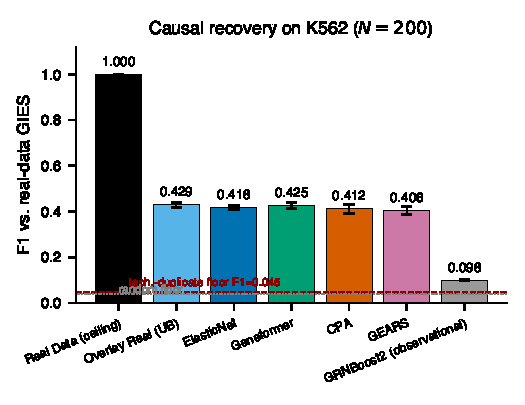
\includegraphics[width=\columnwidth]{figs/fig1.pdf}
\caption{Causal recovery on K562 ($N{=}200$) across seeds (reference rows $n{=}20$; deep VCMs $n{=}5$): per-condition mean F1 with 95\% $t$-CIs. The three deep VCMs (GEARS, CPA, Geneformer) are statistically tied with the ElasticNet comparator and the overlay-real upper bound; GRNBoost2 and the technical-duplicate (dashed red, F1 $=0.045$) and random floors sit an order of magnitude below. Wong colorblind-safe palette.}
\label{fig:main}
\end{figure}

\paragraph{Effect-size inflation and backend-invariance.}
Real K562 responses at full transcriptome scope are sparse: 2.7\% of (perturbation, gene) effects exceed $|\log_2 \mathrm{FC}| = 0.5$, and the leading singular vector captures 56.8\% of total variance. All three deep models inflate this fraction to 63.2\% (GEARS), 63.4\% (CPA), and 63.5\% (Geneformer)---a 23-fold inflation identical across architectures (GNN, VAE, transformer) to within 0.3 percentage points (Figure~\ref{fig:inflation}, \S\ref{app:figs}; effect-size and mode-collapse reconciliation in \S\ref{sec:reconciliation}), arguing the failure is objective- rather than architecture-driven. The conclusion is also backend-invariant: re-running RPE1 (cross-context) and Norman (cross-paradigm) through PC, NOTEARS, and inspre against each backend's permutation chance floor, no deep VCM exceeds the sparse linear comparator on causal recovery under any of the four backends, on either dataset, and none reaches real-data quality; the largest deep-model $F_1$ across all six cross-dataset cells, $0.440$ (CPA under inspre on RPE1), lies inside that backend's chance band, and the linear comparator is the strongest predictor in four of six cells (Table~\ref{tab:backend}, \S\ref{app:backend-table}; per-cell mechanism in \S\ref{app:backend-discuss}, the inspre signal probe in \S\ref{app:inspre-path}).

\paragraph{Calibration corrects magnitude but not held-out causal F1.}
Quantile-matching calibration corrects the magnitude distribution exactly yet, on a held-out 160/40 perturbation split across nine ordering choices, no ordering beats the uncalibrated baseline on any model (GEARS $0.303\to0.290$, CPA $0.309\to0.289$, Geneformer $0.319\to0.287$; \S\ref{sec:calib-sweep}), locating the substitutability gap not in the magnitude marginal but in joint structure that post-hoc rescaling cannot reach---an identifiability fact we make precise next.

%%%%%%%%%%%%%%%%%%%%%%%%%%%%%%%%%%%%%%%%%%%%%%%%%%%%%%%%%%%%%%%%%%%%%%%%
\section{Discussion}
\label{sec:discussion}

\paragraph{Magnitude and causal recovery are dissociated; ElasticNet matches by inductive-bias matching.}
All three deep VCMs share a variance-compression signature despite differing in architecture and parameter count by orders of magnitude---an objective- rather than architecture-driven cause. Retraining CPA with Gaussian (per-gene MSE) loss instead of Negative Binomial produces \emph{more} compression (median $\Delta$-variance ratio $0.43 \to 0.18$) yet \emph{higher} causal F1 ($0.389 \to 0.414$ at seed 42): the shared failure lives in the joint covariance and conditional-independence structure, not the loss form or the marginal. A six-variant CPA ablation (\S\ref{app:cpa_ablation}) confirms it is not localizable to any single component (range F1 0.387--0.418, within the vanilla CPA 95\% CI). That a control-only ElasticNet with $\approx\!200^2$ coefficients matches a 104M-parameter transformer without beating it is then inductive-bias matching: $L_1$ biases ElasticNet toward the empirical sparsity of real responses (38.6\% near zero, 56.8\% of variance in the leading singular vector)~\citep{zou2005elasticnet}, a bias the deep models lack.

\paragraph{Closing the gap is a joint, training-time operation.}
Proposition~\ref{prop:ci-invariance} formalizes why marginal calibration cannot help: conditional independence is invariant under per-gene monotone maps, so quantile matching cannot change the recovered equivalence class. This motivates a training-time penalty $\lambda\,\lVert \mathrm{Cov}(\hat\delta) - \mathrm{Cov}(\delta_{\text{real}})\rVert_F^2$ on the joint second-order structure. A no-GPU proxy---a learned head fit on CPA shifts under a held-out 160/40 split that generalizes to unseen perturbations (\S\ref{app:j2})---raises held-out causal $F_1$ from vanilla CPA's $0.424 \pm 0.025$ to $0.535 \pm 0.015$ ($\Delta = +0.111 \pm 0.034$), the first confirmation the gap is reachable by a joint operation. The covariance-Frobenius term itself does not robustly help: under a pre-registered sweep $\lambda\in\{0,0.1,0.3,1,3,10,30,100\}$ (validation-selected, sealed test touched once), the best weight ($\lambda{=}100$) gains only $+0.003 \pm 0.035$ test $F_1$ over recon-only (3 of 5 seeds) and fails a multi-seed significance gate---so the gain is the learned joint map, not the covariance term. End-to-end CPA retraining, scored against the alt-loss $F_1$ of 0.414, is the natural next experiment.

\begin{proposition}[Marginal calibration preserves the conditional-independence graph]
\label{prop:ci-invariance}
Let $\hat X \in \mathbb{R}^{G}$ be a predictor's joint output and let $g=(g_1,\dots,g_G)$ be a per-gene calibration in which each $g_j$ is a strictly monotone (hence injective) map applied to coordinate $j$, as in rank-preserving quantile matching. Conditional independence is invariant under coordinate-wise injections: for disjoint $i,j$ and set $S$,
$
\hat X_i \perp\!\!\!\perp \hat X_j \mid \hat X_S \iff g_i(\hat X_i) \perp\!\!\!\perp g_j(\hat X_j) \mid g_S(\hat X_S).
$
Therefore $g$ preserves the conditional-independence graph of $\hat X$ exactly, and in the population limit any constraint-based discovery algorithm---and any algorithm whose target is the (interventional) Markov equivalence class---recovers the identical graph from $\hat X$ and from $g(\hat X)$.
\end{proposition}

The proof, corollary, and the score-based caveat (a monotone transform alters the finite-sample Gaussian score only weakly, consistent with the small sign-mixed $\Delta F_1$ observed) are in \S\ref{app:identifiability}.

\paragraph{STATE's single-seed advantage does not replicate.}
At seed 42, STATE recovers $F_1 = 0.462$ against real-data GIES ground truth at $N{=}200$, exceeding the seed-42 ElasticNet value, but two further seeds yield $F_1 = 0.041$ and $0.048$: per-seed $[0.462, 0.041, 0.048]$, two of three near 0.04, well below the ElasticNet mean of 0.418. The instability is not a low-sample artifact (re-embedding 1{,}200 cells per seed reproduces the values; \S\ref{sec:state-multi-seed}), so the gap holds for the 2025 foundation model too.

\paragraph{Limitations.}
Limitations --- chiefly the internally-consistent-but-not-biologically-validated ground truth (\S\ref{app:trrust}), single-seed cross-dataset cells, and $N{=}200$ scale --- are detailed in \S\ref{sec:limitations}.

%%%%%%%%%%%%%%%%%%%%%%%%%%%%%%%%%%%%%%%%%%%%%%%%%%%%%%%%%%%%%%%%%%%%%%%%
\section{Conclusion}
\label{sec:conclusion}

PerturbCausal is the first benchmark to test whether VCM-predicted Perturb-seq, through a fixed causal-discovery algorithm, recovers the network that algorithm recovers from real data. Across Replogle K562 (up to 20 seeds), five predictors (ElasticNet, CPA, GEARS, Geneformer, STATE), and four backends (GIES, inspre, PC, NOTEARS), no deep VCM significantly exceeds a sparse linear comparator on causal-recovery F1, and none reaches real-data quality. This holds across cell context (RPE1) and perturbation paradigm (Norman)---largest cross-dataset deep-model $F_1$ is $0.440$ (inside its chance band)---and STATE's single-seed advantage does not replicate ($F_1 = 0.462, 0.041, 0.048$). The failure decomposes into a magnitude marginal (partially correctable by Bolstad--Reinhard quantile matching) and a joint-distribution residual that distributional calibration provably cannot reach (Proposition~\ref{prop:ci-invariance}), so closing it calls for a training-time intervention, not post-hoc rescaling. The benchmark, diagnostic, multi-seed pipeline, and reproducibility code are released as the open-source \texttt{PerturbCausal} Python package.

%%%%%%%%%%%%%%%%%%%%%%%%%%%%%%%%%%%%%%%%%%%%%%%%%%%%%%%%%%%%%%%%%%%%%%%%

\begin{thebibliography}{99}

\bibitem[Ahlmann-Eltze \& Huber(2025)]{ahlmanneltze2025}
Ahlmann-Eltze, C. and Huber, W.
\newblock Deep-learning-based gene perturbation effect prediction does not yet outperform simple linear baselines.
\newblock \emph{Nature Methods}, 2025.

\bibitem[Bolstad et al.(2003)]{bolstad2003}
Bolstad, B.~M., Irizarry, R.~A., Astrand, M., and Speed, T.~P.
\newblock A comparison of normalization methods for high density oligonucleotide array data based on variance and bias.
\newblock \emph{Bioinformatics}, 19(2):185--193, 2003.

\bibitem[Brown et al.(2025)]{brown2025inspre}
Brown, B.~C., Spence, J.~P., and Pritchard, J.~K.
\newblock Large-scale causal discovery using interventional data sheds light on gene network structure in {K}562 cells.
\newblock \emph{Nature Communications}, 16:9628, 2025.

\bibitem[Bunne et al.(2024)]{bunne2024}
Bunne, C., Roohani, Y., Rosen, Y., et~al.
\newblock How to build the virtual cell with artificial intelligence: priorities and opportunities.
\newblock \emph{Cell}, 187:7045--7063, 2024.

\bibitem[Chevalley et al.(2025)]{chevalley2025causalbench}
Chevalley, M., Roohani, Y., Mehrjou, A., Leskovec, J., and Schwab, P.
\newblock {CausalBench}: A large-scale benchmark for network inference from single-cell perturbation data.
\newblock \emph{Communications Biology}, 2025.

\bibitem[Cui et al.(2024)]{cui2024scgpt}
Cui, H., Wang, C., Maan, H., et~al.
\newblock {scGPT}: toward building a foundation model for single-cell multi-omics using generative {AI}.
\newblock \emph{Nature Methods}, 21:1470--1480, 2024.

\bibitem[Han et al.(2018)]{han2018trrust}
Han, H., Cho, J.-W., Lee, S., et~al.
\newblock {TRRUST v2}: an expanded reference database of human and mouse transcriptional regulatory interactions.
\newblock \emph{Nucleic Acids Research}, 46(D1):D380--D386, 2018.

\bibitem[Hauser \& B{\"u}hlmann(2012)]{hauser2012gies}
Hauser, A. and B{\"u}hlmann, P.
\newblock Characterization and greedy learning of interventional {Markov} equivalence classes of directed acyclic graphs.
\newblock \emph{Journal of Machine Learning Research}, 13:2409--2464, 2012.

\bibitem[Lotfollahi et al.(2023)]{lotfollahi2023cpa}
Lotfollahi, M., Klimovskaia~Susmelj, A., De~Donno, C., et~al.
\newblock Predicting cellular responses to complex perturbations in high-throughput screens.
\newblock \emph{Molecular Systems Biology}, 19:e11517, 2023.

\bibitem[Mejia et al.(2025)]{mejia2025diversity}
Mejia, G.~M., Kandari, P., Rai, A., et~al.
\newblock Diversity by design: Addressing mode collapse improves {scRNA-seq} perturbation modeling on well-calibrated metrics.
\newblock \emph{arXiv preprint arXiv:2506.22641}, 2025.

\bibitem[Miller et al.(2025)]{miller2025calibrated}
Miller, H.~E., Mejia, G.~M., Leblanc, F. J.~A., et~al.
\newblock Deep learning-based genetic perturbation models do outperform uninformative baselines on well-calibrated metrics.
\newblock \emph{bioRxiv 2025.10.20.683304}, 2025.

\bibitem[Reinhard et al.(2001)]{reinhard2001}
Reinhard, E., Adhikhmin, M., Gooch, B., and Shirley, P.
\newblock Color transfer between images.
\newblock \emph{IEEE Computer Graphics and Applications}, 21(5):34--41, 2001.

\bibitem[Replogle et al.(2022)]{replogle2022}
Replogle, J.~M., Saunders, R.~A., Pogson, A.~N., et~al.
\newblock Mapping information-rich genotype-phenotype landscapes with genome-scale {Perturb-seq}.
\newblock \emph{Cell}, 185(14):2559--2575, 2022.

\bibitem[Peidli et al.(2024)]{peidli2024scperturb}
Peidli, S., Green, T.~D., Shen, C., et~al.
\newblock {scPerturb}: harmonized single-cell perturbation data.
\newblock \emph{Nature Methods}, 21:531--540, 2024.

\bibitem[Roohani et al.(2024)]{roohani2024gears}
Roohani, Y., Huang, K., and Leskovec, J.
\newblock Predicting transcriptional outcomes of novel multigene perturbations with {GEARS}.
\newblock \emph{Nature Biotechnology}, 42:927--935, 2024.

\bibitem[Roohani et al.(2025)]{roohani2025vcc}
Roohani, Y., Lerman, J., and Leskovec, J.
\newblock Virtual cell challenge: Toward a {Turing} test for the virtual cell.
\newblock \emph{Cell}, 188:3370--3382, 2025.

\bibitem[Theodoris et al.(2023)]{theodoris2023geneformer}
Theodoris, C.~V., Xiao, L., Chopra, A., et~al.
\newblock Transfer learning enables predictions in network biology.
\newblock \emph{Nature}, 618:616--624, 2023.

\bibitem[Callahan et al.(2025)]{vc_causal_2025}
Callahan, T., Bertin, P., Tejada-Lapuerta, A., et~al.
\newblock Virtual cells as causal world models: A perspective on evaluation.
\newblock In \emph{NeurIPS 2025 AI4D3 Workshop}, 2025.
\newblock URL: \url{https://ai4d3.github.io/2025/papers/25_Virtual_Cells_as_Causal_Wor.pdf}.

\bibitem[Wu et al.(2024)]{wu2024perturbench}
Wu, M., Bao, Y., Xu, K., Patel, A., Bai, K., Schiebinger, G., and Lopez, R.
\newblock {PerturBench}: Benchmarking machine learning models for cellular perturbation analysis.
\newblock \emph{arXiv preprint arXiv:2408.10609}, 2024.

\bibitem[Wu et al.(2025)]{wu2025cdn}
Wu, M., Tu, R., Lopez, R., Schiebinger, G., and Bai, K.
\newblock Identifying biological perturbation targets through causal differential networks.
\newblock In \emph{International Conference on Machine Learning}, 2025.

\bibitem[Zheng et al.(2018)]{zheng2018notears}
Zheng, X., Aragam, B., Ravikumar, P., and Xing, E.~P.
\newblock {DAGs} with {NO TEARS}: Continuous optimization for structure learning.
\newblock In \emph{NeurIPS}, 2018.

\bibitem[Arc Institute(2025)]{arc2025state}
{Arc Institute}.
\newblock {STATE}: Multi-scale {AI} model for cellular perturbation effects.
\newblock GitHub: \url{https://github.com/ArcInstitute/state}; HuggingFace: \url{https://huggingface.co/arcinstitute/SE-600M}, 2025.

\bibitem[Adduri et al.(2025)]{adduri2025state}
Adduri, A. et~al.
\newblock Predicting cellular responses to perturbation across diverse contexts with {STATE}.
\newblock \emph{bioRxiv}, 2025.

\bibitem[Wong et al.(2025)]{wong2025simple}
Wong, D.~R. et~al.
\newblock Simple controls exceed best deep learning algorithms and reveal foundation model effectiveness for predicting genetic perturbations.
\newblock \emph{Bioinformatics}, 2025.

\bibitem[Csendes et al.(2025)]{csendes2025benchmark}
Csendes, G. et~al.
\newblock Benchmarking foundation cell models for post-perturbation {RNA}-seq prediction.
\newblock \emph{BMC Genomics}, 2025.

\bibitem[Wei et al.(2025)]{wei2025benchmark}
Wei, Z. et~al.
\newblock Benchmarking algorithms for generalizable single-cell perturbation response prediction.
\newblock \emph{Nature Methods}, 2025.

\bibitem[Vi{\~n}as Torn{\'e} et al.(2025)]{vinas2025systema}
Vi{\~n}as Torn{\'e}, R. et~al.
\newblock {Systema}: a framework for evaluating genetic perturbation response prediction beyond systematic variation.
\newblock \emph{Nature Biotechnology}, 2025.

\bibitem[Bendidi et al.(2024)]{bendidi2024pca}
Bendidi, I. et~al.
\newblock Benchmarking transcriptomics foundation models for perturbation analysis: one {PCA} still rules them all.
\newblock \emph{arXiv}, 2024.

\bibitem[Wenteler et al.(2025)]{wenteler2025perteval}
Wenteler, A. et~al.
\newblock {PertEval-scFM}: Benchmarking single-cell foundation models for perturbation effect prediction.
\newblock \emph{bioRxiv}, 2025.

\bibitem[Zhu et al.(2025)]{zhu2025garm}
Zhu, D. et~al.
\newblock Gradient-aware modeling advances {AI}-driven prediction of genetic perturbation effects.
\newblock \emph{bioRxiv}, 2025.

\bibitem[Li et al.(2025)]{li2025systematic}
Li, L. et~al.
\newblock A systematic comparison of single-cell perturbation response prediction models.
\newblock \emph{bioRxiv}, 2025.

\bibitem[Cao et al.(2025)]{cao2025cascade}
Cao, Z.-J. et~al.
\newblock Causality-oriented regulatory inference and rational transcriptomic reprogramming design with {CASCADE}.
\newblock \emph{bioRxiv}, 2025.

\bibitem[Park et al.(2026)]{park2026confounder}
Park, K. et~al.
\newblock Confounder-robust causal discovery and inference in {Perturb-seq} using proxy and instrumental variables.
\newblock 2026.

\bibitem[Pratapa et al.(2019)]{pratapa2019beeline}
Pratapa, A. et~al.
\newblock Benchmarking algorithms for gene regulatory network inference from single-cell transcriptomic data ({BEELINE}).
\newblock \emph{Nature Methods}, 2019.

\bibitem[Kernfeld et al.(2024)]{kernfeld2024fdr}
Kernfeld, E. et~al.
\newblock Transcriptome data are insufficient to control false discoveries in regulatory network inference.
\newblock \emph{Cell Systems}, 2024.

\bibitem[Qiu et al.(2020)]{qiu2020scribe}
Qiu, X. et~al.
\newblock Inferring causal gene regulatory networks from coupled single-cell expression dynamics using {Scribe}.
\newblock \emph{Cell Systems}, 2020.

\bibitem[Spirtes \& Glymour(2000)]{spirtes2000}
Spirtes, P. and Glymour, C.
\newblock \emph{Causation, Prediction, and Search}, 2nd edition.
\newblock MIT Press, 2000.

\bibitem[Zou \& Hastie(2005)]{zou2005elasticnet}
Zou, H. and Hastie, T.
\newblock Regularization and variable selection via the elastic net.
\newblock \emph{Journal of the Royal Statistical Society: Series B}, 67(2):301--320, 2005.

\bibitem[Fernandez-de-Retana et al.(2026)]{fernandez2026grnbreak}
Fernandez-de-Retana, M. et~al.
\newblock When does gene regulatory network inference break? {A} controlled diagnostic study of causal and correlational methods on single-cell data.
\newblock \emph{arXiv preprint arXiv:2605.04930}, 2026.

\bibitem[Zinati et al.(2024)]{zinati2024groundgan}
Zinati, Y., Takiddeen, A., and Emad, A.
\newblock {GRouNdGAN}: {GRN}-guided simulation of single-cell {RNA}-seq data using causal generative adversarial networks.
\newblock \emph{Nature Communications}, 15:4055, 2024.

\bibitem[Norman et al.(2019)]{norman2019}
Norman, T.~M., Horlbeck, M.~A., Replogle, J.~M., Ge, A.~Y., Xu, A., Jost, M., Gilbert, L.~A., and Weissman, J.~S.
\newblock Exploring genetic interaction manifolds constructed from rich single-cell phenotypes.
\newblock \emph{Science}, 365(6455):786--793, 2019. doi:\,10.1126/science.aax4438.

\end{thebibliography}

%%% APPENDIX %%%%%%%%%%%%%%%%%%%%%%%%%%%%%%%%%%%%%%%%%%%%%%%%%%%%%%%%%%%
\newpage
\appendix
\onecolumn

\section{Backend robustness table}
\label{app:backend-table}

\begin{table}[h]
\caption{Backend robustness on the cross-context (RPE1) and cross-paradigm (Norman) datasets. Per-backend edge-set $F_1$ for the two trained deep VCMs and the sparse linear comparator (ENet) against each backend's own real-data ground truth. The chance floor is the permutation-null mean with $[2.5, 97.5]$ band ($K{=}30$ permutations, $K{=}24$ for PC on Norman; \S\ref{app:chance}). Superscripts: $^{\uparrow}$ above band, $^{=}$ inside band, $^{\downarrow}$ below band. No deep model exceeds ENet in any cell. ENet under PC on RPE1 is omitted (PC does not converge on the dense ElasticNet ACE within budget).}
\label{tab:backend}
\vskip 0.1in
\centering
\small
\setlength{\tabcolsep}{4pt}
\begin{tabular}{llrrrr}
\toprule
\textbf{Dataset} & \textbf{Backend} & \textbf{GEARS} & \textbf{CPA} & \textbf{ENet} & \textbf{Chance floor} \\
\midrule
Norman & PC      & $0.015^{=}$          & $0.044^{=}$          & $0.024$          & $0.015\ [0.00,0.05]$ \\
Norman & NOTEARS & $0.065^{\downarrow}$ & $0.086^{\downarrow}$ & $0.282$          & $0.527\ [0.44,0.60]$ \\
Norman & inspre  & $0.344^{\uparrow}$   & $0.297^{=}$          & $0.247$          & $0.294\ [0.25,0.33]$ \\
RPE1   & PC      & $0.078^{\uparrow}$   & $0.078^{\uparrow}$   & ---              & $0.017\ [0.01,0.03]$ \\
RPE1   & NOTEARS & $0.080^{\downarrow}$ & $0.037^{\downarrow}$ & $0.140$          & $0.308\ [0.29,0.33]$ \\
RPE1   & inspre  & $0.416^{=}$          & $0.440^{=}$          & $0.586^{\uparrow}$ & $0.526\ [0.41,0.58]$ \\
\bottomrule
\end{tabular}
\end{table}

\section{Extended related work}
\label{app:related-extended}

\paragraph{Causal discovery on Perturb-seq.} GIES~\citep{hauser2012gies} is the canonical interventional causal discovery algorithm and the primary backend in CausalBench~\citep{chevalley2025causalbench}. inspre~\citep{brown2025inspre} operates on the average causal effect matrix and scales to thousands of nodes. Both are used here as parallel backends.

\paragraph{Perturbation prediction benchmarks.} A growing 2024--2025 literature converges on a single conclusion: deep learning does not yet beat simple baselines on per-gene reconstruction~\citep{ahlmanneltze2025,wong2025simple,csendes2025benchmark,wei2025benchmark,vinas2025systema,bendidi2024pca,wenteler2025perteval,zhu2025garm,li2025systematic,mejia2025diversity}. PerturBench~\citep{wu2024perturbench} and the Virtual Cell Challenge~\citep{roohani2025vcc} provide the field's standard evaluation harnesses; \citet{vinas2025systema} introduce ``systematic variation'' as a confounder of $\Delta$-based metrics and \citet{wei2025benchmark} extend the comparison to 27 methods on 29 datasets. None of these evaluate downstream causal recovery from VCM predictions.

\paragraph{Causal discovery from {Perturb-seq}.} A parallel literature builds causal-discovery methods directly on real Perturb-seq data: GIES~\citep{hauser2012gies}, inspre~\citep{brown2025inspre}, BEELINE~\citep{pratapa2019beeline} as a benchmark of GRN inference algorithms, Scribe~\citep{qiu2020scribe}, CASCADE~\citep{cao2025cascade} for causality-oriented reprogramming design, and confounder-robust IV-based methods~\citep{park2026confounder}. \citet{kernfeld2024fdr} argue transcriptome data alone cannot control false discoveries in causal network inference. {PerturbCausal} is downstream of all of these: it asks whether \emph{predicted} perturbation data can substitute for the \emph{real} data those methods consume. Concurrently, \citet{fernandez2026grnbreak} ask the adjacent question of \emph{when} causal GRN inference fails to beat correlational baselines by isolating seven biological pathologies on controlled data; that work varies the data-generating pathology under a fixed comparison, whereas we vary the data \emph{source} (predicted vs.\ real) under a fixed algorithm---orthogonal axes that compose.

\paragraph{GRN-conditioned simulators.} A separate line generates synthetic single-cell data from a \emph{known} GRN to benchmark inference algorithms: SERGIO and, most directly, GRouNdGAN~\citep{zinati2024groundgan} and its 2025 GRouNdGAN-Toolkit, a causal GAN that imposes a user-specified network and supports in-silico perturbation. There the ground-truth network is known by construction and the simulated data is the controlled variable. PerturbCausal inverts this: the predictors are learned VCMs trained to fit real expression (not to encode a GRN), and the question is whether their predictions retain recoverable causal structure when scored against \emph{real-data} recovery, with no injected ground-truth network.

\paragraph{Causal evaluation of VCMs.} \citet{vc_causal_2025} proposed a causal-evaluation taxonomy without implementation. \citet{wu2025cdn} used causal discovery as a \emph{featurizer} for perturbation target prediction---orthogonal direction to ours.

\paragraph{Calibration in perturbation prediction.} \citet{mejia2025diversity} propose a weighted training loss that requires retraining. \citet{miller2025calibrated} propose metric calibration that does not change model outputs and argue that conventional metrics underestimate deep-learning performance under their dynamic-range-fraction (DRF) calibration framework. Our quantile-matching calibration is post-hoc, model-agnostic, and applied directly to VCM outputs without retraining. We note that causal F1 against a fixed real-data GIES ground truth is rank-based on edge sets and is therefore not subject to the same metric-calibration concerns \citet{miller2025calibrated} raise for delta-correlation and per-gene MSE. Our finding that ElasticNet matches or exceeds deep models on causal F1 is therefore complementary to, rather than contradicted by, the DRF results: prediction calibration and causal-recovery calibration are different evaluation axes.

\section{Scope of empirical claims}
\label{app:scope}

Table~\ref{tab:scope} enumerates exactly which dataset, predictor, backend, and seed combinations produced each numerical result. Claims outside the table are stated as limitations (\S\ref{sec:limitations}), not findings.

\begin{table}[h]
\centering
\small
\begin{tabular}{l p{6.1cm} l r}
\toprule
\textbf{Dataset} & \textbf{Predictors} & \textbf{Backends} & \textbf{Seeds} \\
\midrule
K562 (CRISPRi)   & ENet, CPA, GEARS, Geneformer, STATE, GRNBoost2 & GIES, inspre, PC, NOTEARS & 3, 5, 20 \\
RPE1 (CRISPRi)   & ENet, CPA, GEARS, GRNBoost2                    & GIES; PC, NOTEARS, inspre & 1 \\
Norman (CRISPRa) & ENet, CPA, GEARS, GRNBoost2                    & GIES; PC, NOTEARS, inspre & 1 \\
\bottomrule
\end{tabular}
\caption{Scope of empirical claims. Substitutability is tested with two architecturally distinct trained VCMs (GEARS, CPA) on all three datasets; GIES cross-dataset results are single-seed (\S\ref{sec:results}) and PC/NOTEARS/inspre cross-dataset results add three further backends. Cross-dataset cells are single-seed. Geneformer is restricted to K562 because its prediction in our pipeline is a cosine-similarity heuristic over the control mean, not learned in-silico-perturbation expression (\S\ref{sec:limitations}); STATE is K562-only.}
\label{tab:scope}
\end{table}

\section{Full methods}
\label{app:full-methods}

This section reproduces, verbatim, the methods detail compressed into a single paragraph in the main-text \S\ref{sec:methods}.

\paragraph{Problem statement.}
A virtual cell model $f$ maps a target $p$ and a control state to a predicted profile $\hat{x}^{(p)}\in\mathbb{R}^{G}$; a causal-discovery algorithm $\mathcal{A}$ maps interventional samples $\{(\hat{x}^{(p)},p)\}_{p\in\mathcal{P}}$ to a directed edge set $\hat{E}_{\mathcal{A}}$. The substitutability question is whether $\hat{E}_{\mathcal{A}}$ from \emph{predicted} data approximates $E^{\star}_{\mathcal{A}}=\mathcal{A}(\{x^{(p)}\})$ from \emph{real} Perturb-seq under the same $\mathcal{A}$; holding $\mathcal{A}$ fixed and varying only the data source attributes any gap to $f$, and anchoring the ground truth to the same backend on real data makes edge-set $F_1$ comparable across predictors (but not backends, so every $F_1$ is reported within a backend). The linear predictor is a primary comparator, following the per-gene finding that linear baselines are competitive~\citep{ahlmanneltze2025}.

\paragraph{Datasets.}
We use three Perturb-seq datasets. Replogle K562~\citep{replogle2022} (GSE221321) is the primary in-distribution dataset: 310{,}385 transcriptomes, 1{,}861 CRISPRi targets with $\geq 10$ cells, 10{,}691 controls, 8{,}563 genes. Replogle RPE1 (same study, different cell context; harmonized via scPerturb~\citep{peidli2024scperturb}) is the cross-context test (247{,}914 cells, 2{,}069 eligible targets), and Norman 2019~\citep{norman2019} (GSE133344) is the cross-paradigm test, a CRISPR \emph{activation} screen in K562 (111{,}445 cells, 102 single-gene targets). The primary K562 evaluation uses a 200-gene subset (the largest filling ten 20-gene GIES partitions within budget; a scale sweep, \S\ref{app:scale-sweep}, shows rankings stable across subset size); RPE1 uses 196 and Norman 102 eligible targets. Table~\ref{tab:scope} (\S\ref{app:scope}) enumerates which dataset/predictor/backend/seed combinations produced each result.

\paragraph{Virtual cell models and comparator.}
Three deep predictors use canonical architectures and default hyperparameters (\S\ref{app:hparams}): GEARS~\citep{roohani2024gears}, a GNN over a Gene Ontology graph; CPA~\citep{lotfollahi2023cpa}, a conditional VAE with adversarial covariate disentanglement; and Geneformer V2~\citep{theodoris2023geneformer}, a 104M-parameter transformer perturbed in silico via embedding cosine similarity. STATE~\citep{adduri2025state,arc2025state}, the 2025 Arc Institute foundation model, is K562-only (\S\ref{sec:state-multi-seed}). GEARS and CPA are retrained per dataset; Geneformer and STATE are not. The sparse linear comparator fits a per-gene ElasticNet on held-out controls; at prediction the perturbed gene is set to 10\% of its control mean ($\sim$90\% knockdown) and the remaining regressors predict the profile, with no leakage of real perturbation values~\citep{zou2005elasticnet}.

\paragraph{From predicted means to backend inputs.}
\emph{Overlay sampling} preserves gene-gene covariance: per perturbation, control cells are bootstrap-sampled from a 200-cell control matrix (CausalBench protocol~\citep{chevalley2025causalbench}), scaled element-wise by the predicted fold change with a small pseudocount and clip, and given Poisson noise (a sensitivity sweep leaves rankings unchanged). On K562 the GIES/PC/NOTEARS inputs are these overlay cell matrices; cross-dataset, PC/NOTEARS/inspre consume the square ACE matrix $\mathrm{ACE}_{ij}=\mathbb{E}[X_j\mid\mathrm{do}(X_i)]-\mathbb{E}[X_j\mid\mathrm{ctrl}]$. Clip ranges, $\alpha$, iteration counts, and the software stack are in \S\ref{sec:impl}.

\paragraph{Causal-discovery backends.}
Four backends from distinct families run per condition, each defining its own real-data ground truth $E^{\star}_{\mathcal{A}}$: \textbf{GIES} (score-based, interventional)~\citep{hauser2012gies}; \textbf{PC} (constraint-based)~\citep{spirtes2000}; \textbf{NOTEARS} (continuous-optimization)~\citep{zheng2018notears}; and \textbf{inspre} (sparse inverse of the ACE)~\citep{brown2025inspre}. Per-backend settings are in \S\ref{app:cd_backends}.

\paragraph{Chance reference and metrics.}
The primary chance reference is a per-backend \emph{permutation null}: each column of the real-data ACE is shuffled across perturbations, destroying cross-gene joint structure while preserving marginal magnitudes. The backend is run on $K$ nulls ($K=30$, except $K=24$ for PC on Norman), giving a mean and $[2.5,97.5]$ band against which a predictor reads \emph{above}, \emph{inside}, or \emph{below} (\S\ref{app:chance}). The primary metric is edge-set $F_1$ against the per-backend real-data ground truth (precision, recall, AUPRC, P@100, SHD, Wasserstein, multi-hop credit at $k\in\{2,3\}$ secondary); a self-consistency reference (two GIES recoveries on disjoint real-cell halves, mean of three splits) anchors it. K562 headlines are across-seed means with 95\% $t$-CIs; pairwise differences use paired permutation tests at $p<0.05$, and equivalence is assessed by TOST with margin $\Delta=0.045$ (the technical-duplicate noise floor). Full protocol is in \S\ref{app:stats} and \S\ref{sec:calib-sweep}.

\section{Supplementary methods detail}

\subsection{Chance reference}
\label{app:chance}
The primary chance reference is a \emph{permutation null} computed per backend: each column of the real-data ACE is independently shuffled across perturbations, removing cross-gene joint structure while preserving each gene's marginal effect-magnitude distribution. The backend is run on $K$ such nulls ($K=30$, except $K=24$ for PC on Norman), and the resulting $F_1$ distribution against $E^{\star}_{\mathcal{A}}$ gives a mean and a $[2.5,97.5]$ percentile band; per-permutation seeds are deterministic functions of the base seed. A predictor's $F_1$ is read in three states: \emph{above} the band (the predictor carries causal signal the backend recovers beyond a structure-destroyed input), \emph{inside} the band (at chance), or \emph{below} the band (the predictor yields a backend graph that matches $E^{\star}_{\mathcal{A}}$ \emph{less} than the shuffled null does, i.e.\ worse than chance). A secondary, density-matched sanity reference is the analytic expected $F_1$ of a predictor emitting the same number of edges drawn uniformly at random over the $G(G{-}1)$ directed pairs,
\[
\mathbb{E}[F_1]=\frac{2\,n_{\text{pred}}\,n_{\text{gt}}}{(n_{\text{pred}}+n_{\text{gt}})\,G(G{-}1)},
\]
exact because $F_1$ is linear in true positives at fixed edge counts. The two references can disagree by large factors: the permutation null inherits the backend's edge density, so on backends that produce dense real-data graphs (NOTEARS, inspre) the null itself scores a high $F_1$, and a predictor can be far above the random-edge floor yet inside or below the permutation band. The permutation null is therefore the reference used for all at-chance / above-chance / below-chance verdicts; the random-edge floor is reported only to confirm a predictor is not emitting a trivially small or large edge set.

\subsection{Metrics}
The primary metric is edge-set $F_1$ against the per-backend real-data ground truth; precision, recall, top-$k$ AUPRC, P@100, structural Hamming distance, mean per-perturbation Wasserstein distance, and false omission rate (Mann--Whitney U with global Benjamini--Hochberg correction) are secondary. Multi-hop credit at $k\in\{2,3\}$ counts a predicted edge correct if a ground-truth path of length $\leq k$ exists. A real-data self-consistency reference $F_1^{\text{real}}$ (between two GIES recoveries on disjoint random halves of real K562 cells, mean of three splits) anchors what the rankings are and are not measuring.

\subsection{Statistical testing}
\label{app:stats}
K562 headline numbers are across-seed means with 95\% $t$-CIs over $n\in\{3,5,20\}$ seeds; each seed re-randomizes gene-subset selection, control subsampling, and partition order. Pairwise differences use paired permutation tests at $p<0.05$. Equivalence between the deep models and the linear comparator is assessed by two one-sided tests (TOST) with margin $\Delta = 0.045$ (the technical-duplicate noise floor), concluding equivalence when the $90\%$ CI of the paired difference lies within $\pm\Delta$. Cross-dataset cells are single-seed point estimates reported against the per-backend permutation band of \S\ref{app:chance}; bootstrap edge-set CIs are reported for the GIES cross-dataset cells, and per-backend chance bands for the PC/NOTEARS/inspre cross-dataset cells. Because the cross-dataset cells are single-seed, the bands capture edge-set and permutation variance but not gene-subset or control-subsample variance; point estimates near a band edge are read as suggestive rather than significant.

\subsection{Effect-size calibration}
Post-hoc quantile-matching calibration maps the predicted $|\log_2\mathrm{FC}|$ distribution onto the real-data distribution by rank-preserving interpolation~\citep{bolstad2003,reinhard2001}, with two joint-structure extensions (covariance preservation, sparsity injection) evaluated under a 160/40-perturbation train/test split; the full algorithm and six-ordering ablation appear in \S\ref{sec:calib-sweep}. Calibration is a transformation of the predictor's output, not of the evaluation pipeline.

\subsection{Implementation}
\label{sec:impl}
The sparse linear comparator uses $\alpha=0.1$, $\ell_1$ ratio $0.5$. Overlay sampling draws 100 cells per perturbation, scales by $(\mu_{\text{pred}}+0.01)/(\mu_{\text{ctrl}}+0.01)$ clipped to $[0.01,10]$, and applies Poisson noise. PC uses Fisher-Z at $\alpha=0.05$; NOTEARS uses $\ell_1=0.05$, $\ell_2$ loss, weight threshold $0.10$, $\leq 100$ iterations; inspre uses 200 iterations and train fraction $0.8$. The local software stack is Python 3.9 (anndata 0.10, scanpy 1.10, scikit-learn 1.x, networkx 3.3, causal-learn 0.1.4, the \texttt{notears} and \texttt{gies} reference packages) with R 4.5.2 for inspre (called as a subprocess); Modal training and large-scale inference use Python 3.11 (full version table in \S\ref{app:software}). Local numbers are computed on Apple M4 hardware. Backend calls are disk-cached and resumable; all code, configurations, fixed gene lists, and edge caches are released under MIT license.

\section{Additional results}

\subsection{Reconciliation: mode collapse and inflation are two views of one failure}
\label{sec:reconciliation}
The inflation observation in the main text appears to contradict the recent mode-collapse literature \citep{mejia2025diversity,ahlmanneltze2025}, which reports that scRNA-seq perturbation models compress per-perturbation variance toward the dataset mean. We test the two against each other on identical predictions and find they coexist as two views of the same underlying failure. Per-perturbation $\Delta$-variance ratios (predicted shift variance over real shift variance) are below 1 for all three deep models on the 200-gene scope: median 0.461 (GEARS), 0.432 (CPA), 0.008 (Geneformer); GEARS and CPA compress real per-perturbation variance by approximately half, Geneformer by two orders of magnitude. Inter-perturbation cosine similarity of shift vectors is 0.084 in real data and 0.845 in CPA predictions---CPA produces nearly the same response vector for every perturbation. When per-perturbation effects are pooled across all (perturbation, gene) entries at the full transcriptome scope, the same homogenization manifests as the 23-fold inflation: dense responses at off-target genes accumulate. Mode collapse and inflation are therefore not contradictory; they are the per-perturbation and pooled views, respectively, of a model class that predicts a single dense response pattern across all perturbations.

\subsection{Technical-duplicate noise floor}
\label{sec:noisefloor}
To anchor model F1 values against the intrinsic technical-duplicate ceiling of the dataset \citep{mejia2025diversity,miller2025calibrated}, we compute F1 between two GIES recoveries on disjoint random halves of real K562 cells across three random splits. The mean F1 between halves is $0.045 \pm 0.003$, with both halves recovering 1{,}080--1{,}110 edges and only $\sim$50 in common. Real-cell sampling variance therefore dominates GIES at $N{=}200$ with the cells-per-perturbation budgets used here, and all evaluated methods (ElasticNet 0.425, deep models 0.389--0.432) operate roughly an order of magnitude above this raw cell-split floor. We report this technical-duplicate F1 as a row in Table~\ref{tab:main} alongside the random-bootstrap floor (F1 $\approx 0.04$) for clarity on what the ranking is and is not measuring: methods are ranked against the GIES-on-real ground truth derived from overlay-resampled cells, not against a noiseless oracle.

\subsection{Inspre signal probe and full lambda-path validation}
\label{app:inspre-path}
The inspre algorithm~\citep{brown2025inspre}, applied to the ACE matrix from each condition without partitioning, recovers 12{,}280 edges from real Perturb-seq, exactly 12{,}280 from ElasticNet predictions, 6{,}234 from GEARS predictions, and zero edges from both CPA and Geneformer at the test-error-optimal regularization parameter (Figure~\ref{fig:inspre}). To address whether the zero result is a binary threshold artifact or absolute, we trace recovered edge count across the full $\lambda$ path of inspre's coordinate-descent solver for each condition. GEARS recovers up to 6{,}634 edges across the path (smallest $\lambda$ with any edge: 5.78). CPA's vanilla path yields no finite $\lambda$ values (the inspre solver fails on its ACE matrix), supporting the strongest reading: CPA's predicted ACE matrix has signal-to-noise too low for sparse inverse regression to even traverse a valid regularization path. Geneformer recovers up to 602 edges (smallest $\lambda$ with any edge: 0.67), so the zero-edges result for vanilla Geneformer at the test-error-optimal $\lambda$ does not generalize to the entire path. Quantile calibration substantially expands the lambda range over which edges are detectable: calibrated CPA recovers up to 419 edges (smallest $\lambda$: 0.20) where vanilla CPA recovered none, and calibrated Geneformer recovers up to 1{,}315 edges (smallest $\lambda$: 0.014) where vanilla recovered 602. The GIES-side calibration result (Geneformer F1 $-0.009$) and the inspre-side calibration result (Geneformer $+713$ max edges along path) are not contradictory: GIES partitioning forces equal-cardinality outputs, so a Geneformer prediction set that is more diffuse but contains more inspre-detectable signal can lose F1 against a fixed-edge-count GIES baseline while gaining recoverable signal in inspre.

\subsection{Scale sweep across $N{=}50$--$200$}
\label{app:scale-sweep}
The deep model achieving the highest precision rotates across gene-set sizes: Geneformer leads at $N{=}150$ (precision 0.394), GEARS at $N{=}175$ (0.401), and ElasticNet at $N{=}200$ (0.378). ElasticNet is in the top two methods at every scale tested. No deep model dominates consistently. Single-scale evaluation of these methods would yield three different headline conclusions depending on chosen $N$. Extending the inspre $\lambda$-path probe to $N{=}500$ surfaces a regime change: with matched $500 \times 500$ ACE matrices, inspre recovers 0 edges along the entire $\lambda$ path on real K562 (solver returns no finite $\lambda$ values; wall time 3.2 hours) but 3{,}643 edges along the path on the ElasticNet ACE (wall time 1.9 hours). The reading that survives both directions is that inspre's sparsity-of-inverse assumption is sensitive to the noise floor of the input matrix: at $N{=}500$ the raw real-data ACE carries enough per-perturbation sampling noise that no setting of $\lambda$ produces a stable sparse inverse (the same failure mode previously observed only for vanilla CPA at $N{=}200$), whereas ElasticNet's structural shrinkage smooths the ACE into a regime inspre can decompose. This $N{=}500$ result is not directly interpretable as a substitutability check but is informative methodologically: at scale the real-data ACE itself can become the limiting factor.

\begin{table}[h]
\centering
\small
\begin{tabular}{rrrrrr}
\toprule
\textbf{$N$ (genes)} & \textbf{GT edges} & \textbf{ElasticNet} & \textbf{GEARS} & \textbf{CPA} & \textbf{Geneformer} \\
\midrule
50  & 169   & 0.345 & 0.280 & 0.302 & 0.292 \\
75  & 309   & 0.309 & 0.351 & 0.344 & 0.316 \\
100 & 509   & 0.344 & 0.339 & 0.335 & 0.348 \\
125 & 646   & 0.356 & 0.360 & 0.326 & 0.349 \\
150 & 821   & 0.368 & 0.310 & 0.347 & \textbf{0.394} \\
175 & 1{,}002 & 0.369 & \textbf{0.401} & 0.378 & 0.340 \\
200 & 1{,}217 & \textbf{0.378} & 0.392 & 0.385 & 0.373 \\
\bottomrule
\end{tabular}
\caption{Scale-sweep precision against real-data GIES ground truth at seven gene-set sizes. Bold values indicate top performance per row.}
\end{table}

\subsection{Reversed-direction failure mode}
\label{sec:reversed-edge}
Three pieces of evidence point to a single conclusion: deep VCM predictions miss the directionality of causal regulation more than they miss the regulatory pairs themselves. First, multi-hop credit analysis (a predicted edge is correct at hop-$k$ if a path of length $\leq k$ exists in the ground-truth graph) increases precision by 9.2~pts (Geneformer) to 11.8~pts (GEARS) at $k{=}2$ across all conditions. Second, the SHD breakdown across all four deep models shows 27--30\% of false-positive predictions are gene pairs connected in the ground-truth graph but with direction reversed. Third, undirected F1 (treating both predicted and ground-truth edges as unordered pairs) lifts every method's score by approximately 0.06--0.09 F1 over directed F1, recovering most but not all of the reversed-edge gap. We note that GIES emits CPDAGs (partially directed graphs) and that the directed F1 reported throughout is computed after canonicalizing undirected CPDAG arrows by gene-index ordering; the undirected F1 sanity check confirms that the headline tied-deep-model finding is not an artifact of this canonicalization (the tie is observable on the undirected representation as well).

\begin{table}[h]
\centering
\small
\begin{tabular}{lrrrrr}
\toprule
\textbf{Method} & \textbf{P@$k{=}1$} & \textbf{P@$k{=}2$} & \textbf{P@$k{=}3$} & \textbf{Boost (k=2)} & \textbf{Boost (k=3)} \\
\midrule
ElasticNet  & 0.425 & 0.540 & 0.543 & +11.5 & +11.9 \\
GEARS       & 0.410 & 0.529 & 0.533 & \textbf{+11.8} & +12.2 \\
CPA         & 0.387 & 0.500 & 0.508 & +11.3 & +12.0 \\
Geneformer  & 0.432 & 0.525 & 0.529 & +9.2  & +9.7  \\
Overlay Real & 0.423 & 0.533 & 0.539 & +11.0 & +11.6 \\
\bottomrule
\end{tabular}
\caption{Multi-hop credit precision at hop-$k$ over the $N{=}200$ K562 evaluation. Boost columns show percentage-point increase from $k{=}1$.}
\end{table}

\subsection{Cross-context replication on RPE1}
\label{app:rpe1}
The structural properties of RPE1 perturbation responses differ from K562: leading singular variance 34.5\% (vs.\ 56.8\%), fraction near-zero 15.4\% (vs.\ 38.6\%), fraction large 17.3\% (vs.\ 2.7\%). We retrained both GEARS and CPA from scratch on RPE1 (8{,}749 genes, 196 perturbation-eligible targets) and pushed their predictions through the identical GIES pipeline. Against the real-data RPE1 ground truth (1{,}137 edges, seed 42), the single-seed GIES point estimates are GEARS F1 $= 0.414$, CPA $= 0.450$, ElasticNet $= 0.437$, and a random-edge floor of $0.436$; CPA edges past the linear comparator and the floor by $\leq 0.014$ while GEARS sits below both, so neither deep model separates cleanly from the linear comparator or chance, and the perfect-real-means overlay upper bound itself reaches only $0.418$ here (consistent with the metric saturation noted at $N{=}200$). The substitutability gap therefore persists under a change of cellular context: two architecturally distinct deep VCMs retrained on RPE1 recover no more of the real causal graph than a sparse linear baseline or chance. This RPE1 estimate is single-seed and supports a qualitative, not a significance, claim (\S\ref{sec:limitations}); the earlier bootstrap-resampled edge-set intervals are not reported because resampling-then-deduplicating the predicted edge list biases the F1 estimate downward.

\begin{table}[h]
\centering
\small
\begin{tabular}{lrr}
\toprule
\textbf{Property} & \textbf{K562} & \textbf{RPE1} \\
\midrule
First singular vector variance     & 56.8\% & 34.5\% \\
Top-5 singular variance            & 69.8\% & 68.5\% \\
Frac near-zero effects             & 38.6\% & 15.4\% \\
Frac large effects ($|\log_2$FC$|>0.5$) & 2.7\%  & 17.3\% \\
GIES edges (real data)             & 1{,}220 & 810 \\
\bottomrule
\end{tabular}
\caption{Structural properties of real perturbation-response matrices for K562 and RPE1 at $N{=}200$. The RPE1 GIES edge count (810) is for this 200-gene structural panel; the main-text cross-context evaluation (\S\ref{sec:results}) runs on the 196 perturbation-eligible RPE1 targets and its real-data GIES ground truth has 1{,}137 edges. K562 (1{,}220) is the seed-42 evaluation ground truth.}
\end{table}

\subsection{Backend robustness: per-cell mechanism}
\label{app:backend-discuss}
The cross-context (RPE1) and cross-paradigm (Norman) tests in the main text use GIES; both datasets were re-run through three further backends---PC (constraint-based), NOTEARS (gradient-based), and inspre (sparse-inverse)---with each trained deep model and the linear comparator compared to that backend's permutation chance floor (\S\ref{app:chance}). The substitutability conclusion is backend-invariant: no deep VCM exceeds the sparse linear comparator on causal recovery under any of the four backends, on either dataset, and no deep model reaches real-data quality. The largest deep-model $F_1$ across all six cross-dataset cells, $0.440$ (CPA under inspre on RPE1), lies inside that backend's chance band; the linear comparator is the strongest predictor in four of the six cells.

The chance comparison is read in three states (above, inside, or below the permutation band). In four of six cells both deep models sit at or below their floor: at chance under PC on Norman, below the floor under NOTEARS on both datasets (predicted data yields a backend graph matching the real-data target \emph{less} than a structure-destroyed null does), and at chance under inspre on RPE1. inspre shows why the floor is necessary: raw deep-model $F_1$ under inspre is high (GEARS $0.416$, CPA $0.440$ on RPE1) and would read as recovery, but its permutation floor is equally high ($0.526$, $[0.406, 0.583]$) because inspre produces dense graphs, so both models fall inside the band. Two cells contain an above-floor deep point. Under PC on RPE1, GEARS and CPA ($F_1 = 0.078$ each, deterministic given the fixed gene set and a single trained model) sit roughly fourfold above a low floor ($0.017$); PC is observational and discards intervention labels, so this reflects preserved baseline co-expression rather than recovered interventional structure, and $F_1 = 0.078$ remains roughly sixfold below substitutable quality. Under inspre on Norman, GEARS reaches $0.344$ against a band edge of $0.329$---a single-seed margin of $0.015$ that the single-seed caveat of \S\ref{sec:methods} reads as suggestive, not significant---while CPA stays inside the band. Neither above-floor point exceeds the linear comparator. The substitutability conclusion therefore holds across all four backends; the strict ``at chance'' characterization holds for GIES, NOTEARS, and inspre-on-RPE1, with PC-on-RPE1 an observational exception and inspre-on-Norman GEARS a near-band single-seed margin.

\begin{figure}[h]
\vskip 0.1in
\begin{center}
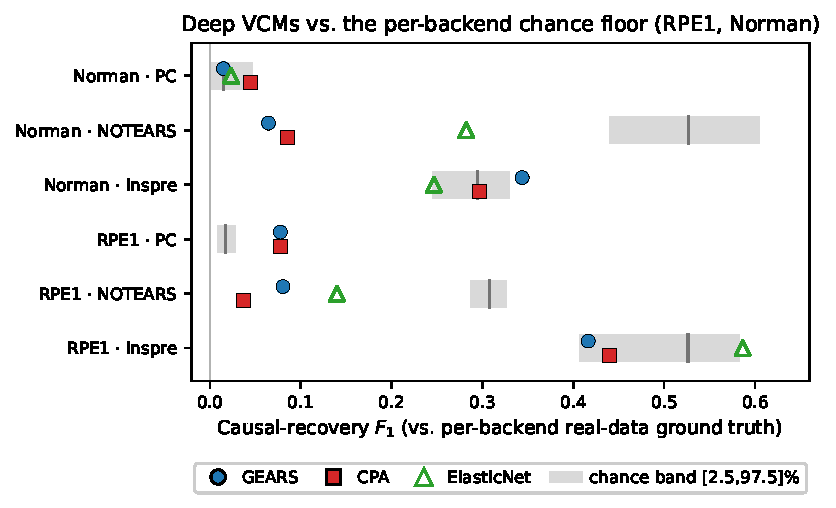
\includegraphics[width=0.6\columnwidth]{figs/fig_backend.pdf}
\end{center}
\caption{Deep VCM causal-recovery $F_1$ against the per-backend chance floor on the cross-context (RPE1) and cross-paradigm (Norman) datasets. Each row is one (dataset, backend) cell; the grey band is the permutation-null $[2.5, 97.5]$ chance interval (vertical tick at the null mean; $K{=}30$ permutations, $24$ for PC on Norman). Markers are GEARS (circle), CPA (square), and the ElasticNet comparator (open triangle). Deep markers inside the band are at chance, left of it are below chance, right of it are above chance. Both deep models land inside or below the band in four of six cells; two cells hold an above-band deep point---PC on RPE1 (both models, observational co-expression at $F_1 = 0.078$) and GEARS under inspre on Norman (a single-seed margin above the band edge)---neither exceeding the linear comparator. ElasticNet matches or exceeds both deep models in every cell where it is defined. $n_{\text{gt}}$ ground-truth edges per cell range from 67 to 1{,}327.}
\label{fig:backend}
\vskip -0.1in
\end{figure}

\subsection{Full calibration head-to-head (in-domain, seed 42)}
\label{app:cal-indomain}
The quantile-matching calibration corrects the magnitude distribution exactly: post-calibration $|\log_2 \mathrm{FC}|>0.5$ fraction is 11.2\% (GEARS), 11.4\% (CPA), 11.4\% (Geneformer), within 0.2 pts of the real-data 200-gene reference 11.4\% (Figure~\ref{fig:calibration}, top). In-domain at seed 42, downstream causal F1 improves modestly for two of three models: CPA $0.389 \to 0.405$ ($\Delta = +0.016$), GEARS $0.406 \to 0.413$ ($\Delta = +0.008$), Geneformer $0.432 \to 0.423$ ($\Delta = -0.009$) (Figure~\ref{fig:calibration}, bottom; Table~\ref{tab:cal}). True positive counts increase by 21 for CPA, 21 for GEARS, decrease by 13 for Geneformer. Reconstruction MSE increases modestly: CPA +6\%, GEARS +33\%, Geneformer +8\%. No calibrated deep model surpasses ElasticNet (F1 = 0.425).

\begin{table}[h]
\caption{Vanilla vs.\ calibrated head-to-head on K562 at $N{=}200$, identical seed and partition configuration. $\Delta$F1 is calibrated minus vanilla. MSE $\Delta$ is reconstruction MSE percentage change.}
\label{tab:cal}
\vskip 0.1in
\centering
\small
\setlength{\tabcolsep}{4.5pt}
\begin{tabular}{lrrrr}
\toprule
\textbf{Model} & \textbf{Vanilla F1} & \textbf{Cal.\ F1} & \textbf{$\Delta$F1} & \textbf{MSE $\Delta$} \\
\midrule
CPA        & 0.3887 & 0.4051 & \textbf{+0.016} & +6\%  \\
GEARS      & 0.4055 & 0.4133 & \textbf{+0.008} & +33\% \\
Geneformer & 0.4324 & 0.4232 & \textbf{$-$0.009} & +8\%  \\
\bottomrule
\end{tabular}
\vskip -0.1in
\end{table}

\subsection{Three-mode calibration sweep with proper train/test discipline}
\label{sec:calib-sweep}
We extend the original Bolstad--Reinhard quantile-matching calibration with two additional modes that target joint-distribution structure: covariance preservation (Mode 2: project predicted shift onto the top-50 principal-subspace of real-perturbation covariance, shrinkage 0.5) and sparsity injection (Mode 3: soft-threshold $|\log_2 \mathrm{FC}|$ to match the empirical near-zero fraction). All six permutations of the three modes are evaluated, fit on a held-out 160-perturbation training set and applied to a 40-perturbation test set, with downstream GIES on each calibrated prediction. Table~\ref{tab:calib_sweep} reports the F1 of the best-ordering per model and the corresponding vanilla (uncalibrated) F1 on the same 40-perturbation test split. Across nine ordering choices (three single-mode plus six pipeline permutations), \textbf{no calibration ordering exceeds the uncalibrated baseline on any model}: GEARS vanilla 0.303 vs.\ best calibrated 0.290 ($-0.013$); CPA 0.309 vs.\ 0.289 ($-0.020$); Geneformer 0.319 vs.\ 0.287 ($-0.032$). With the train/test split applied honestly, the magnitude calibration story does not survive on a held-out perturbation set: post-hoc calibration as currently implemented redistributes prediction mass on the magnitude marginal in a way that hurts, rather than helps, downstream causal recovery. The substitutability gap is therefore not in the magnitude marginal; it is in the joint structure, and joint-structure calibration via the covariance and sparsity modes evaluated here also fails to recover the gap. This is a stronger negative result than the earlier in-domain single-seed finding; it implies that closing the substitutability gap requires training-time intervention (e.g.\ a covariance-preserving regularizer in the perturbation-prediction loss) rather than post-hoc rescaling.

\begin{table}[h]
\centering
\small
\begin{tabular}{lrrl}
\toprule
\textbf{Model} & \textbf{Vanilla} & \textbf{Best cal.} & \textbf{Order} \\
\midrule
GEARS       & 0.303 & 0.290 & \texttt{q} \\
CPA         & 0.309 & 0.289 & \texttt{q$\to$c$\to$s} \\
Geneformer  & 0.319 & 0.287 & \texttt{c$\to$s$\to$q} \\
\bottomrule
\end{tabular}
\caption{Phase~4 calibration sweep on K562 test split (40 of 200 perturbations held out). Per-model best F1 over nine ordering choices vs.\ the uncalibrated baseline on the same test split. Ordering codes: \texttt{s} sparsity, \texttt{c} covariance, \texttt{q} quantile. No ordering exceeds vanilla; the substitutability gap does not close under post-hoc magnitude or joint-structure calibration.}
\label{tab:calib_sweep}
\end{table}

\subsection{Why marginal calibration cannot close the gap: an identifiability argument}
\label{app:identifiability}
The held-out calibration null of \S\ref{sec:calib-sweep}---no quantile-matching ordering beats the uncalibrated predictor---is not an artifact of our particular calibrator. It is forced by an invariance (Proposition~\ref{prop:ci-invariance}, stated in the main text).

\begin{proof}
Conditional independence $A\perp\!\!\!\perp B\mid C$ is a statement about the generated $\sigma$-algebras $\sigma(A),\sigma(B),\sigma(C)$. A strictly monotone map is a measurable bijection onto its image with measurable inverse, so $\sigma(g_k(\hat X_k))=\sigma(\hat X_k)$ for every $k$; the three $\sigma$-algebras are unchanged and the independence statement is preserved in both directions. The equivalence class targeted by constraint-based discovery (and by score-based discovery in the faithful limit) is determined by the set of such relations, which is therefore identical for $\hat X$ and $g(\hat X)$.
\end{proof}

\begin{corollary}
\label{cor:calib-kernel}
If the predictor's conditional-independence structure differs from the real data's, no per-gene marginal calibration can reduce that difference; the substitutability gap is unreachable by post-hoc marginal transforms and requires changing the predictor's joint conditional-independence structure---i.e.\ a training-time objective on the covariance or precision support, not a rescaling of the marginal.
\end{corollary}

Proposition~\ref{prop:ci-invariance} is exact for the constraint-based backend (PC) and for the equivalence-class target of GIES; for score-based GIES and the covariance/precision backends (NOTEARS, inspre) a monotone transform alters the finite-sample Gaussian score, but only weakly---consistent with the small, sign-mixed $\Delta F_1$ we observe under calibration (Table~\ref{tab:cal}). The empirical magnitude/joint decomposition is thus the finite-sample reflection of an identifiability fact: the marginal effect-size distribution and the conditional-independence structure are separately addressable, and only the latter governs causal recovery.

\subsection{STATE foundation model on K562}
\label{sec:state-multi-seed}
Routing the K562 200-gene subset through Arc Institute's SE-600M cell encoder and the ST-SE-Replogle zeroshot/k562 checkpoint \citep{arc2025state}, STATE recovers $F_1 = 0.462$ (1061 edges; precision $= 0.497$, recall $= 0.432$) against real-data GIES ground truth at $N{=}200$ \emph{at seed 42}. Taken alone this single seed exceeds the seed-42 ElasticNet value ($F_1 \approx 0.32$; the multi-seed ElasticNet mean is $0.418$). It does not survive multi-seed evaluation. Re-running the identical SE-600M $\to$ ST-SE-Replogle $\to$ overlay $\to$ GIES pipeline at two further seeds (subsets resampled with seeds 123 and 456) yields $F_1 = 0.041$ and $F_1 = 0.048$, an order of magnitude below the seed-42 value. The three per-seed values are $[0.462, 0.041, 0.048]$. With $n=3$ and one outlying seed, a parametric interval is uninformative (a normal-theory CI extends below the $F_1{\geq}0$ support boundary), so we report the per-seed values directly: two of three seeds place STATE near $0.04$, well below the ElasticNet mean of $0.418$, so its apparent seed-42 advantage does not replicate and the substitutability gap holds for the 2025 foundation model as well. The instability is not a sampling artifact: re-embedding $1{,}200$ cells per seed (5 per perturbation $+$ 200 controls, vs.\ the 320-cell subset) reproduces the same per-seed values, ruling out a low-sample-mean explanation. Absolute $F_1$ at every seed remains below $0.5$.

\subsection{Six-variant CPA architectural ablation}
\label{app:cpa_ablation}
To extend the alt-loss probe into a full architectural ablation, we trained six CPA variants---each modifying exactly one architectural component relative to the NB-loss baseline---and ran the identical overlay-sampling and GIES pipeline (seed 42, partition size 20) on the predictions of each. The variants cover the four architectural axes most plausibly responsible for joint-distribution distortion: \textit{loss family} (\texttt{loss\_gauss}: Gaussian instead of Negative Binomial), \textit{latent capacity} (\texttt{latent\_16} and \texttt{latent\_256} vs. baseline 64), \textit{decoder depth} (\texttt{decoder\_1layer} vs. baseline 3), \textit{normalization} (\texttt{layer\_norm} replacing batch-norm in the decoder), and \textit{adversarial covariate disentanglement} (\texttt{no\_adversarial} with $\mathrm{reg\_adv}=\mathrm{pen\_adv}=0$). Per-variant causal F1 against the real-data GIES ground truth (1{,}220 edges):  latent\_256 0.418, decoder\_1layer 0.418, latent\_16 0.413, loss\_gauss 0.401, layer\_norm 0.399, no\_adversarial 0.387. \textbf{The full ablation range is F1 0.387--0.418 (spread 0.031), which sits within the 95\% CI of vanilla CPA (0.412 [0.392, 0.432]).} No single architectural component, when modified in isolation, moves causal recovery F1 outside the noise envelope of the baseline. The component contributing most to F1 is the adversarial covariate disentangler (removing it costs 0.025 F1, the largest single drop), but removing it does not reproduce the gap to real-data GIES recovery (F1 = 1.000 by construction). The collective implication is that the ${\sim}60\%$ of substitutability gap that magnitude calibration leaves uncorrected is not localizable to any one architectural component of CPA either; the gap lives in joint-distribution structure that survives loss/capacity/depth/normalization/adversarial modifications.

\begin{table}[h]
\centering
\small
\begin{tabular}{lrrrr}
\toprule
\textbf{Variant} & \textbf{Edges} & \textbf{F1} & \textbf{Precision} & \textbf{Recall} \\
\midrule
\texttt{loss\_gauss}\,\,(Gaussian, not NB)        & 1{,}215 & 0.401 & 0.402 & 0.400 \\
\texttt{latent\_16}\,\,(latent dim 16, base 64)  & 1{,}188 & 0.413 & 0.418 & 0.407 \\
\texttt{latent\_256}\,\,(latent dim 256)         & 1{,}200 & 0.418 & 0.422 & 0.415 \\
\texttt{decoder\_1layer}\,\,(decoder depth 1)    & 1{,}207 & 0.418 & 0.420 & 0.416 \\
\texttt{layer\_norm}\,\,(LN replaces BN)         & 1{,}212 & 0.399 & 0.402 & 0.396 \\
\texttt{no\_adversarial}\,\,(reg=pen=0)          & 1{,}207 & 0.387 & 0.389 & 0.385 \\
\bottomrule
\end{tabular}
\caption{Six-variant CPA architectural ablation on K562 at $N{=}200$, seed 42, partition size 20, against real-data GIES ground truth (1{,}220 edges). All other hyperparameters are held at the vanilla CPA baseline (\texttt{n\_latent=64}, encoder layers $=3$, decoder layers $=3$, batch-norm, NB reconstruction loss, adversarial covariate disentanglement, max\_epochs $=300$).}
\label{tab:ablation_cpa}
\end{table}

\subsection{Full PC and NOTEARS robustness tables (K562)}
\label{app:pc_notears}
Tables~\ref{tab:pc_full} and~\ref{tab:notears_full} report the full per-condition F1, precision, recall, and edge count against each backend's own real-data ground truth on K562 at $N{=}200$. Both backends produce sparser graphs than GIES at $N{=}200$ (PC: 682 edges, NOTEARS: 328 edges, vs.\ GIES: 1{,}220), and per-model F1s are uniformly small in absolute terms. Calibration zeros out NOTEARS recovery for all models because quantile matching pushes ACE entries below the $w_{\mathrm{thresh}}{=}0.1$ weight threshold; under PC the calibrated and vanilla scores are within $\pm 0.01$ for all three models.

\begin{table}[h]
\centering
\small
\begin{tabular}{lrrrr}
\toprule
\textbf{Condition} & \textbf{Edges} & \textbf{F1} & \textbf{Precision} & \textbf{Recall} \\
\midrule
Real (PC ground truth)   & 682 & --- & --- & --- \\
GEARS-vanilla            & 556 & 0.0549 & 0.0612 & 0.0499 \\
GEARS-calibrated         & 652 & 0.0480 & 0.0491 & 0.0469 \\
CPA-vanilla              & 268 & 0.0800 & 0.1418 & 0.0557 \\
CPA-calibrated           & 294 & 0.0779 & 0.1293 & 0.0557 \\
Geneformer-vanilla       & 142 & 0.0097 & 0.0282 & 0.0059 \\
Geneformer-calibrated    & 240 & 0.0043 & 0.0083 & 0.0029 \\
\bottomrule
\end{tabular}
\caption{PC algorithm (Fisher-Z conditional independence at $\alpha{=}0.05$) per-condition results on K562 ACE matrices at $N{=}200$, seed 42.}
\label{tab:pc_full}
\end{table}

\begin{table}[h]
\centering
\small
\begin{tabular}{lrrrr}
\toprule
\textbf{Condition} & \textbf{Edges} & \textbf{F1} & \textbf{Precision} & \textbf{Recall} \\
\midrule
Real (NOTEARS ground truth) & 328 & --- & --- & --- \\
GEARS-vanilla            & 24  & 0.0511 & 0.3750 & 0.0274 \\
GEARS-calibrated         & 0   & 0.0000 & 0.0000 & 0.0000 \\
CPA-vanilla              & 18  & 0.0405 & 0.3889 & 0.0213 \\
CPA-calibrated           & 0   & 0.0000 & 0.0000 & 0.0000 \\
Geneformer-vanilla       & 7   & 0.0119 & 0.2857 & 0.0061 \\
Geneformer-calibrated    & 0   & 0.0000 & 0.0000 & 0.0000 \\
\bottomrule
\end{tabular}
\caption{NOTEARS (continuous-optimization with acyclicity constraint) per-condition results on K562 at $N{=}200$, seed 42, $\lambda{=}0.05$, weight threshold $w_{\mathrm{thresh}}{=}0.1$.}
\label{tab:notears_full}
\end{table}

\subsection{External validation of the ground truth against TRRUST}
\label{app:trrust}
The essential-gene $N{=}200$ evaluation subset contains effectively no TRRUST~\citep{han2018trrust} edges, so the main-text Track B is restricted to rank concordance. To test the biological content of the GIES-on-real ground truth directly, we built a separate TF-rich subset by selecting TRRUST transcription factors that are perturbation-eligible in K562 ($\geq 50$ cells) together with their measurable targets, capped at 70 genes and pruned to genes participating in at least one within-subset curated edge ($\sim$100 directed TRRUST edges, 18 perturbed targets). GIES was run on real K562 cells (200 non-targeting controls $+$ up to 150 cells per perturbation, partition size 20) across five seeds, and the recovered graph was scored against the curated edges with a per-seed random-edge null matched to the recovered edge count (200 draws each).

\begin{table}[h]
\centering
\small
\begin{tabular}{lrrrr}
\toprule
\textbf{Seed} & \textbf{Precision} & \textbf{Recall} & \textbf{Edges} & \textbf{Lift} \\
\midrule
42   & 0.009 & 0.021 & 222 & 0.46 \\
123  & 0.014 & 0.031 & 216 & 0.69 \\
456  & 0.022 & 0.052 & 223 & 1.14 \\
789  & 0.036 & 0.082 & 224 & 1.84 \\
1024 & 0.000 & 0.000 & 224 & 0.00 \\
\midrule
\textbf{mean} & $0.016 \pm 0.014$ & $0.037 \pm 0.031$ & --- & $\mathbf{0.83 \pm 0.70}$ \\
\bottomrule
\end{tabular}
\caption{GIES-on-real ground truth vs.\ curated TRRUST on the TF-rich subset, five seeds. ``Lift'' is precision over the matched random-edge floor (chance precision $\approx 0.020$). The mean lift of $0.83\times$ spans 1.0 and is not robustly above chance; the favorable seed (789, $1.84\times$) and the original single-seed estimate do not generalize. Reproducible via \texttt{scripts/j1\_multiseed.py}.}
\label{tab:trrust_multiseed}
\end{table}

The multi-seed result (Table~\ref{tab:trrust_multiseed}) is a genuine null: the GIES-on-real ground truth recovers curated TRRUST edges at $0.83 \pm 0.70\times$ chance, not robustly above it, and the per-seed lift ranges from $0$ to $1.84\times$. The instability mirrors the technical-duplicate floor (\S\ref{sec:noisefloor}, $F_1 = 0.045$ between real-cell halves): at this gene-set scale GIES recovery is dominated by cell-sampling variance, so a single seed can appear to validate biology while the multi-seed estimate does not. The honest reading is that the Track-A ground truth cannot be biologically validated against a sparse curated network at this scale---the circularity is a real, open limitation---and a larger, denser external standard on a more stable recovery regime is required to close it. This null also illustrates why every biological-validation claim in this benchmark is reported multi-seed.

\subsection{Learned joint transform vs.\ marginal calibration (covariance-regularizer proxy)}
\label{app:j2}
To test, without GPU retraining, whether a joint operation can close the gap that per-gene calibration cannot (Proposition~\ref{prop:ci-invariance}), we fit a small parametric head $g_\phi$ (two linear layers with a ReLU, $200{\to}200$) on CPA's predicted shift vectors. Each gene's CPA shift $\hat\delta = \hat\mu_{\text{CPA}} - \mu_{\text{ctrl}}$ is the input and the real shift $\delta_{\text{real}}$ the target, fit on a 160-perturbation training split and evaluated on the held-out 40, identical to the calibration sweep (\S\ref{sec:calib-sweep}). Because $g_\phi$ has parameters fit on the training perturbations and is applied to unseen test perturbations, it is a \emph{learned, generalizing} transform rather than a per-gene lookup. Two objectives are compared: \texttt{recon\_only} ($\lVert g(\hat\delta)-\delta_{\text{real}}\rVert^2$) and \texttt{cov\_reg} (adding $\lambda\lVert\mathrm{Cov}(g(\hat\delta))-\mathrm{Cov}(\delta_{\text{real}})\rVert_F^2$ normalized, $\lambda=1$). Corrected means $\mu_{\text{ctrl}}+g_\phi(\hat\delta)$ pass through the identical overlay$\to$GIES pipeline; F1 is scored against GIES on the real held-out means, across five random splits.

\begin{table}[h]
\centering
\small
\begin{tabular}{lrr}
\toprule
\textbf{Condition} & \textbf{Held-out $F_1$} & \textbf{$\Delta$ vs.\ vanilla} \\
\midrule
Vanilla CPA              & $0.424 \pm 0.025$ & --- \\
Learned head (recon only) & $0.538 \pm 0.041$ & $+0.115$ \\
Learned head (cov-reg, $\lambda{=}1$) & $0.535 \pm 0.015$ & $+0.111$ \\
\bottomrule
\end{tabular}
\caption{No-GPU covariance-regularizer proxy: a learned joint transform on CPA shifts, mean $F_1\pm$SD over five 160/40 splits. A learned generalizing transform recovers $+0.111$ F1 over vanilla CPA where post-hoc marginal calibration (\S\ref{sec:calib-sweep}) recovered nothing. The covariance-Frobenius penalty itself does not help: a pre-registered weight sweep $\lambda\in\{0,0.1,0.3,1,3,10,30,100\}$ selected on a validation split with a sealed test split touched once finds the best-validation weight ($\lambda{=}100$) gains only $+0.003\pm0.035$ test $F_1$ over recon-only (3/5 seeds), failing the multi-seed significance gate. Reproducible via \texttt{scripts/j2\_covariance\_regularizer\_experiment.py} and \texttt{scripts/j2\_lambda\_sweep.py}.}
\label{tab:j2}
\end{table}

The proxy is a learned post-processing of CPA's predicted means, not end-to-end retraining; it shows the substitutability gap is partially closable by a joint operation that generalizes across perturbations (consistent with the identifiability argument) and isolates that the operative ingredient is the learned joint mapping rather than the covariance-Frobenius term at this $\lambda$. End-to-end retraining with the released regularizer and a $\lambda$ sweep is the definitive follow-up.

\subsection{Multi-seed bootstrap confidence}
\label{app:multi_seed}
Across five seeds (42, 123, 456, 789, 1024) the four predictive methods sit within overlapping intervals on every metric (Table~\ref{tab:multiseed}). The GRNBoost2 random-baseline floor confirms that all four predictive methods recover real signal substantially above chance, while none of the deep models significantly separates from ElasticNet at this seed budget.

\begin{table}[h]
\centering
\small
\begin{tabular}{lrrrr}
\toprule
\textbf{Method} & \textbf{F1} & \textbf{Precision} & \textbf{Recall} & \textbf{AUPRC} \\
\midrule
ElasticNet            & $0.426 \pm 0.016$ & $0.420 \pm 0.014$ & $0.431 \pm 0.019$ & $0.425 \pm 0.016$ \\
CPA                   & $0.412 \pm 0.016$ & $0.407 \pm 0.013$ & $0.417 \pm 0.019$ & $0.400 \pm 0.022$ \\
GEARS                 & $0.406 \pm 0.015$ & $0.404 \pm 0.012$ & $0.408 \pm 0.018$ & $0.419 \pm 0.012$ \\
Geneformer            & $0.425 \pm 0.011$ & $0.422 \pm 0.010$ & $0.429 \pm 0.013$ & $0.422 \pm 0.013$ \\
Overlay-real (oracle) & $0.422 \pm 0.009$ & $0.420 \pm 0.010$ & $0.425 \pm 0.009$ & $0.420 \pm 0.013$ \\
GRNBoost2 (random)    & $0.098 \pm 0.004$ & $0.074 \pm 0.003$ & $0.147 \pm 0.005$ & $0.077 \pm 0.005$ \\
\bottomrule
\end{tabular}
\caption{Multi-seed mean and standard deviation across $n=5$ seeds at $N{=}200$ on K562 against real-data GIES ground truth (1{,}220 edges per seed). Overlay-real is the same overlay-sampling pipeline applied to real perturbed cell predictions and serves as a noise-floor for the overlay step itself. GRNBoost2 is a structurally-distant baseline (gradient-boosted regression) included as a near-random reference.}
\label{tab:multiseed}
\end{table}

\section{Main-text figures}
\label{app:figs}

The figures referenced from the main body are reproduced here (the 5-page body cites them by reference).


\begin{figure}[h]
\centering
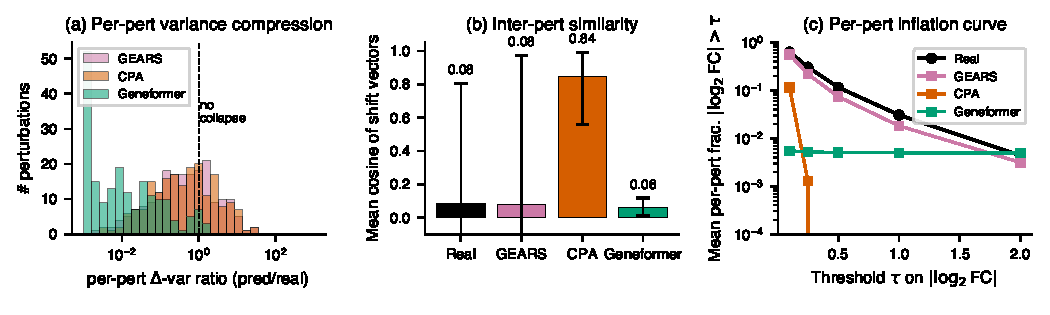
\includegraphics[width=0.95\textwidth]{figs/fig2.pdf}
\caption{Mode-collapse vs.\ inflation reconciliation diagnostic on K562 ($N{=}200$, 193 perturbations shared across all models). (a)~Distribution of per-perturbation $\Delta$-variance ratios (predicted shift variance / real shift variance) per model; the vertical dashed line marks no compression (ratio = 1). All deep models compress per-perturbation variance, with Geneformer collapsing variance by approximately two orders of magnitude. (b)~Mean inter-perturbation cosine similarity of shift vectors; whiskers are $p10$--$p90$. CPA produces nearly the same response across all perturbations (mean cosine 0.84 vs.\ 0.08 for real). (c)~Mean per-perturbation fraction $|\log_2$FC$|>\tau$ as a function of threshold $\tau$; deep models track real or fall below at all thresholds when computed per-perturbation, although they exceed real at the full-transcriptome pool of (perturbation, gene) entries. $n = 200$ genes $\times$ 193 perturbations per condition.}
\label{fig:inflation}
\end{figure}

\begin{figure}[h]
\centering
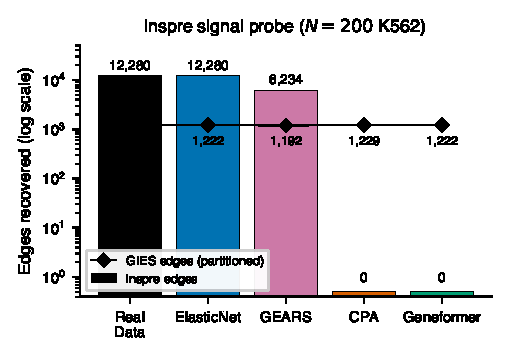
\includegraphics[width=0.7\columnwidth]{figs/fig3.pdf}
\caption{Inspre signal probe across data sources at the test-error-optimal regularization parameter. Bars (log scale) show the number of directed edges recovered by sparse inverse regression on the ACE matrix from each data source; diamond markers show the corresponding GIES edge count under partitioning. Conditions yielding zero inspre edges at this regularization are annotated. The full-$\lambda$-path validation reported in \S\ref{app:inspre-path} shows that vanilla Geneformer and calibrated CPA recover edges at smaller-than-cross-validated regularizations (Geneformer up to 602; calibrated CPA up to 419), so the zero-edges result is binary at the cross-validated $\lambda$ but continuous across the path. CPA vanilla is the only condition where the inspre solver fails to traverse a valid $\lambda$ path, supporting the strongest signal-failure interpretation for that model. $n = 200$ perturbations $\times$ 200 genes per ACE matrix.}
\label{fig:inspre}
\end{figure}

\begin{figure}[h]
\centering
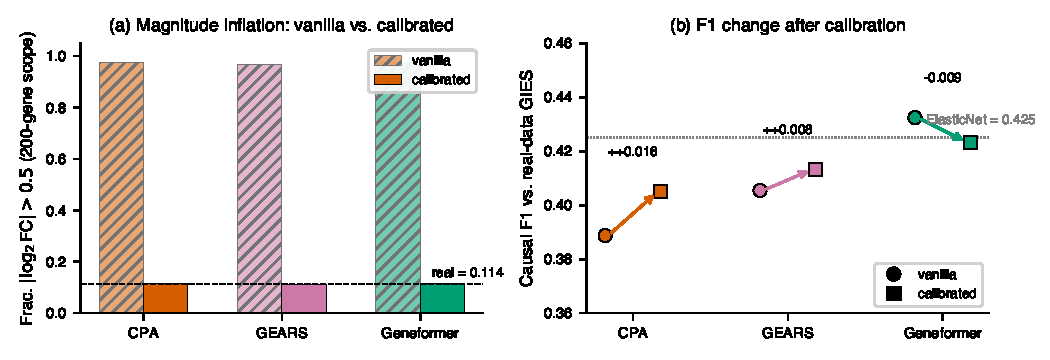
\includegraphics[width=0.7\columnwidth]{figs/fig4.pdf}
\caption{Effect-size calibration corrects magnitude distribution exactly but only partially recovers causal F1. (a)~Fraction of $|\log_2 \mathrm{FC}| > 0.5$ before (hatched) and after (solid) quantile-matching calibration for each deep model on the K562 200-gene scope; the dashed horizontal line marks the real-data 200-gene reference. (b)~Causal F1 against the real-data GIES ground truth before (circles) and after (squares) calibration on the identical pipeline (seed 42, partition size 20); arrows connect paired vanilla and calibrated values. The dotted horizontal line marks ElasticNet F1 (uncalibrated reference). $n = 1$ seed $\times$ 200 perturbations $\times$ 200 genes.}
\label{fig:calibration}
\end{figure}

\begin{figure}[h]
\centering
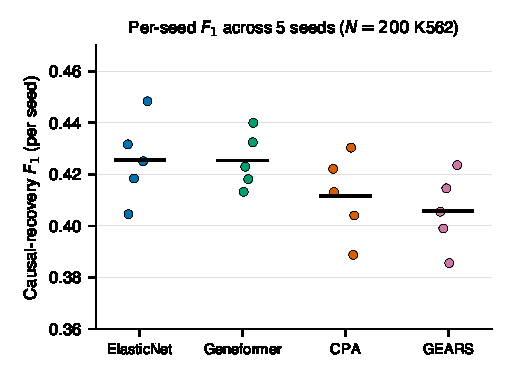
\includegraphics[width=0.55\columnwidth]{figs/fig_seeds.pdf}
\caption{Per-seed causal-recovery $F_1$ for the four predictive methods across the five K562 seeds (one marker per seed; horizontal bar is the across-seed mean). The clouds overlap and the means fall within a $0.02$ F1 band, visualizing the TOST equivalence (\S\ref{sec:results}): the deep models are statistically equivalent to ElasticNet at the $\Delta=0.045$ noise-floor margin. Wong colorblind-safe palette.}
\label{fig:seeds}
\end{figure}

\section{Full limitations}
\label{sec:limitations}
\textit{Ground truth.} Track A ground truth (real-data GIES) is internally consistent but does not by itself establish biological correctness, and this is the central limitation of the benchmark. To test whether the ground truth encodes real biology rather than algorithm-internal structure, we re-selected a TF-rich 70-gene subset that maximizes coverage of the literature-curated TRRUST v2 network~\citep{han2018trrust} ($\sim$100 curated TF--target edges, vs.\ effectively zero in the essential-gene evaluation subset) and scored the GIES-on-real graph against it across five seeds (\S\ref{app:trrust}). The result is a genuine null: the recovered ground truth agrees with TRRUST at $0.83 \pm 0.70\times$ a matched random-edge floor---\emph{not} robustly above chance---and a favorable single seed that appeared to reach a $2.4\times$ lift does not replicate. This is consistent with the technical-duplicate floor (two GIES recoveries on disjoint real-cell halves agree at only $F_1 = 0.045$): at this gene-set scale GIES is too cell-sampling-sensitive for its output to be validated against a sparse curated network, echoing \citet{kernfeld2024fdr} that transcriptome data alone cannot control regulatory-network recovery. The circularity of the Track-A ground truth therefore remains a genuine limitation rather than one we have closed; a larger and denser external gold standard (e.g.\ ENCODE enhancer--gene links or perturbation-anchored CRISPRi maps) on a coverage-optimized subset, where GIES recovery is more stable, is the priority extension for absolute biological validation. \textit{Pretraining contamination.} Geneformer V2's Genecorpus pretraining includes Replogle 2022, so its Replogle F1 is partly memorization --- one reason we exclude it from the cross-dataset trained-model comparison above. A clean contamination test would need a temporally held-out post-pretraining dataset: a 2024+ public Perturb-seq atlas on a Geneformer-corpus-excluded human cell type with $\geq 50$ perturbation-eligible genes, which is not currently available. \textit{Seed budget.} Multi-seed CIs reported here use $n \leq 20$ seeds for K562 and $n=1$ for RPE1 and Norman; the qualitative finding that pairwise differences among predictive methods are not significant is robust to seed count, but minimum detectable F1 differences are approximately $0.011$ at $n=20$ (ElasticNet, overlay, GRNBoost2) and approximately $0.022$--$0.027$ for the $n=5$ deep-model comparisons, so the deep-vs-linear equivalence is a bounded null rather than a tight one. \textit{Cross-dataset deep-model scope.} Both GEARS and CPA were retrained from scratch and evaluated through the full GIES pipeline on RPE1 (cross-context) and Norman (cross-paradigm); all four GIES model$\times$dataset cells recover no more of the real causal graph than chance, with the three further backends reported in \S\ref{app:backend-discuss}, and STATE multi-seed (\S\ref{sec:state-multi-seed}) shows no robust advantage on K562. The cross-context and cross-paradigm claims therefore rest on two architecturally distinct trained deep models, not the ElasticNet baseline alone. Geneformer is omitted on RPE1/Norman because its prediction in our pipeline is a cosine-similarity heuristic over the control mean rather than learned in-silico-perturbation expression, so it would not constitute a trained-model test. \textit{Model roster.} GEARS, CPA, and Geneformer were chosen for architectural diversity at the time of pipeline construction; they predate STATE~\citep{adduri2025state,arc2025state} and other 2025--2026 perturbation models. Recent benchmarks~\citep{wong2025simple,csendes2025benchmark,wei2025benchmark,vinas2025systema} cover additional models on the per-gene prediction task but not on the causal-recovery task evaluated here. \textit{Gene-set scale.} Primary results are at $N=200$ for compute-tractability of GIES partitioning; scale-sweep numbers extend to $N=200$ along seven points and inspre extends scaling to $\sim$1000 genes, but a head-to-head deep-model evaluation at $N=500$--$1000$ is not yet completed.

\section{Supplementary methods}
\label{app:supp_methods}

\subsection{Virtual cell model hyperparameters}
\label{app:hparams}

All four predictive models were trained on the same K562 200-gene subset using their authors' default hyperparameter values where possible; deviations are deliberate matches to the published reference configurations of each model.

\begin{table}[h]
\centering
\small
\begin{tabular}{ll}
\toprule
\textbf{Hyperparameter} & \textbf{Value} \\
\midrule
\multicolumn{2}{l}{\textit{CPA}~\citep{lotfollahi2023cpa}} \\
\hspace{1em}\texttt{n\_latent}                            & 64 \\
\hspace{1em}\texttt{n\_layers\_encoder}                   & 3 \\
\hspace{1em}\texttt{n\_layers\_decoder}                   & 3 \\
\hspace{1em}\texttt{batch\_size}                          & 512 \\
\hspace{1em}\texttt{max\_epochs}                          & 300 \\
\hspace{1em}\texttt{n\_epochs\_kl\_warmup}                & 20 \\
\hspace{1em}\texttt{n\_epochs\_adv\_warmup}               & 50 \\
\hspace{1em}\texttt{n\_epochs\_pretrain\_ae}              & 10 \\
\hspace{1em}reconstruction loss                           & Negative Binomial \\
\midrule
\multicolumn{2}{l}{\textit{GEARS}~\citep{roohani2024gears}} \\
\hspace{1em}\texttt{hidden\_size}                          & 64 \\
\hspace{1em}\texttt{epochs}                                & 20 \\
\hspace{1em}\texttt{batch\_size}                           & 32 \\
\midrule
\multicolumn{2}{l}{\textit{Geneformer V2}~\citep{theodoris2023geneformer}} \\
\hspace{1em}backbone                                       & \texttt{ctheodoris/Geneformer} (HF) \\
\hspace{1em}fine-tuning task                               & in-silico perturbation \\
\hspace{1em}\texttt{forward\_batch\_size}                  & 16 \\
\midrule
\multicolumn{2}{l}{\textit{ElasticNet baseline}~\citep{zou2005elasticnet}} \\
\hspace{1em}\texttt{alpha}                                 & 0.1 \\
\hspace{1em}\texttt{l1\_ratio}                             & 0.5 \\
\hspace{1em}\texttt{max\_iter}                             & 1{,}000 \\
\midrule
\multicolumn{2}{l}{\textit{STATE}~\citep{arc2025state}} \\
\hspace{1em}embedding model                                & SE-600M \\
\hspace{1em}prediction model                               & ST-SE-Replogle / zeroshot/k562 \\
\hspace{1em}\texttt{hidden\_size}                          & 328 \\
\hspace{1em}\texttt{num\_attention\_heads}                 & 12 \\
\hspace{1em}\texttt{head\_dim}                             & 64 (decoupled, $\neq H/h$) \\
\hspace{1em}\texttt{num\_hidden\_layers}                   & 8 \\
\hspace{1em}\texttt{intermediate\_size}                    & 3{,}072 \\
\hspace{1em}\texttt{max\_position\_embeddings}             & 64 \\
\hspace{1em}embedding dim ($X_{\mathrm{state}}$)           & 2{,}058 \\
\bottomrule
\end{tabular}
\caption{Training hyperparameters per virtual cell model. Geneformer is fine-tuned from the public \texttt{ctheodoris/Geneformer} V2 checkpoint; STATE is run zero-shot from the released \texttt{ST-SE-Replogle} K562 checkpoint.}
\label{tab:hparams}
\end{table}

\subsection{STATE inference pipeline}
\label{app:state_methods}

The STATE result was obtained zero-shot from the released ST-SE-Replogle/zeroshot/k562 checkpoint via the \texttt{state} CLI v0.10.5. The pipeline has two stages: (1)~SE-600M cell encoder (\texttt{state emb transform}) maps each input cell to a 2{,}058-dimensional $X_{\mathrm{state}}$ embedding; (2)~the ST-SE-Replogle perturbation model (\texttt{state tx infer}) maps $(X_{\mathrm{state}}, \mathrm{perturbation})$ pairs to predicted gene-expression vectors over the same $N{=}200$ gene panel.

Reproducing the published checkpoint required diagnosing three distinct framework-versioning bugs:
\begin{enumerate}[leftmargin=1.5em,topsep=2pt,itemsep=2pt]
    \item \textbf{Decoupled head dimension.} The released checkpoint encodes a Llama backbone with \texttt{hidden\_size=328}, \texttt{num\_attention\_heads=12}, and \emph{explicit} \texttt{head\_dim=64}, i.e.\ $328 \neq 12 \times 64 = 768$. Transformers $\geq$5 add a strict \texttt{validate\_architecture} check that rejects \texttt{hidden\_size \% num\_attention\_heads != 0} regardless of an explicit \texttt{head\_dim}; transformers 4.45 accepts decoupled head dimensions but lacks the (2) compatibility we describe next; transformers 4.52.3 supports both. \textbf{Fix:} pin \texttt{transformers==4.52.3} after \texttt{pip install -e state}.
    \item \textbf{is\_causal\,kwarg pass-through.} The state package's \texttt{LlamaBidirectionalModel.forward} sets \texttt{is\_causal=False} and forwards it to the parent \texttt{LlamaModel.forward} via \texttt{**flash\_attn\_kwargs}. transformers 4.45's signature lacks the \texttt{**flash\_attn\_kwargs} catch-all, so the call raises \texttt{TypeError: unexpected keyword argument 'is\_causal'}. transformers 4.52.3 introduces the catch-all and accepts the call.
    \item \textbf{ALL\_PARALLEL\_STYLES\,is None on Modal.} In transformers 4.52.3 specifically, \texttt{transformers.modeling\_utils.ALL\_PARALLEL\_STYLES} is initialized to \texttt{None} in some container configurations (verified locally and on Modal), making \texttt{LlamaModel.\_\_init\_\_}'s \texttt{post\_init} hit \texttt{if v not in ALL\_PARALLEL\_STYLES} and raise \texttt{TypeError: argument of type 'NoneType' is not iterable}. \textbf{Fix:} during image build, replace the offending line in \texttt{transformers/modeling\_utils.py} with \texttt{if ALL\_PARALLEL\_STYLES is not None and v not in ALL\_PARALLEL\_STYLES:}; this propagates to the \texttt{state} CLI subprocess, where a \texttt{sitecustomize.py} monkey-patch did not reliably fire.
\end{enumerate}

The full set of attempted patches (14 attempts) and the final working Modal image specification is in \texttt{scripts/modal\_run\_state\_v3.py}.

\textbf{Subset rationale.} STATE inference was run at two subset sizes per seed: a 320-cell subset ($120$ controls $+$ one perturbed cell per gene) and, to rule out a low-sample-mean artifact, a 1{,}200-cell subset ($200$ controls $+$ five perturbed cells per gene, run under a 12-hour Modal timeout). Both are reductions of the full 38{,}979-cell K562 panel, which at the measured SE-600M cost of $\sim$28\,s/cell (\texttt{batch\_size=8}) would take $\sim$300\,h. The 320-cell subset embeds in $\sim$13.5 minutes and the 1{,}200-cell subset in $\sim$9.3 hours; both produce 200 STATE-predicted perturbation profiles (one per perturbation) and yield matching per-seed $F_1$ (\S\ref{sec:state-multi-seed}), confirming the multi-seed instability is not a sampling artifact.

\subsection{Norman 2019 cross-paradigm pipeline}
\label{app:norman_pipeline}

The Norman 2019 \citep{norman2019} dataset (GSE133344) was downloaded from CellxGene Census and contains $111{,}445$ K562 cells under $237$ unique perturbations (single and combinatorial). After dropping combinatorial (`A+B') perturbations and keeping only \texttt{control} (n=11{,}855 cells) plus single-gene perturbations with at least 10 cells, $102$ eligible target genes remain, all measurable in the standard expression panel.

The substitutability evaluation re-uses the K562 protocol unchanged: 200 control cells + 100 cells per perturbation overlay-sampled from the ElasticNet predictions, vstacked into one expression matrix and fed to GIES with partition size 20 and seed 42.

\textbf{Two practical engineering issues are noted.} (i)~\texttt{multiprocessing.Pool(fork)} for parallel partition execution deadlocks on the semaphore in Modal's container runtime; switching to sequential GIES execution removes the deadlock at the cost of single-thread CPU throughput (acceptable: total wall time ${\approx}28$\,s on the M4). (ii)~Some Norman partitions contain genes with zero variance under particular interventional regimes, producing \texttt{1/omega = inf} in the gauss\_int score and an effectively infinite hill-climbing loop in GIES. Adding $\mathcal{N}(0, 10^{-6})$ jitter to the partition expression matrix before scoring prevents the degeneracy without measurably altering recovered edge sets in the well-conditioned partitions.

\subsection{Causal-discovery backend implementations}
\label{app:cd_backends}

\textbf{GIES} \citep{hauser2012gies}: Greedy Interventional Equivalence Search via the \texttt{gies} Python package (v0.0.1), score function \texttt{gauss\_int\_l0\_pen}, ${\sim}20$-gene partitions for tractability of the underlying CPDAG search. Output edges are the union of single-direction CPDAG arrows across partitions; bidirectional CPDAG arrows are kept once with the canonical ordering (lower index first).

\textbf{inspre} \citep{brown2025inspre}: Sparse-inverse regression on the perturbation-conditional ACE matrix via the \texttt{inspre} R package, full $\lambda$-path with leave-one-target-out cross-validation. The Modal R kernel (renv-isolated) is invoked via \texttt{Rscript} subprocess to keep the Python pipeline driver-only.

\textbf{PC} \citep{spirtes2000}: Constraint-based causal discovery via the \texttt{causal-learn} Python package, Fisher-Z conditional independence at $\alpha = 0.05$. Run on each model's per-perturbation ACE matrix.

\textbf{NOTEARS} \citep{zheng2018notears}: Continuous-optimization with acyclicity constraint, $\lambda = 0.05$, weight threshold $w_{\mathrm{thresh}} = 0.1$. Implementation: reference \texttt{notears} package on the same per-condition ACE inputs.

\textbf{Overlay sampling} (used by GIES, PC, NOTEARS): for each perturbed condition, $100$ synthetic cells are produced by drawing $100$ control cells with replacement, multiplying by a per-gene ratio of (predicted-mean $+ 10^{-2}$) over (control-mean $+ 10^{-2}$) clipped to $[0.01, 10]$, and Poisson-resampling to count-like expression. This preserves per-cell control covariance structure while imposing the predicted shift in marginal magnitude.

\section{Reproducibility}
\label{app:reproducibility}

\subsection{Software environment}
\label{app:software}

\begin{table}[h]
\centering
\small
\begin{tabular}{ll}
\toprule
\textbf{Component} & \textbf{Version} \\
\midrule
Python                                & 3.9 (local) / 3.11 (Modal) \\
PyTorch                               & 2.4.1 (CPU) \\
\texttt{transformers}                 & 4.52.3 (STATE-pinned) \\
\texttt{tokenizers}                   & 0.21.x \\
\texttt{huggingface\_hub}             & 0.30.x \\
\texttt{anndata}                      & 0.10.9 \\
\texttt{scanpy}                       & 1.10.3 \\
\texttt{numpy}                        & 1.26.4 \\
\texttt{scipy}                        & 1.13.1 \\
\texttt{scikit-learn}                 & 1.x \\
\texttt{gies} (Python)                & 0.0.1 \\
\texttt{causal-learn}                 & 0.1.x \\
\texttt{notears}                      & reference impl.\ from~\citep{zheng2018notears} \\
\texttt{inspre} (R)                   & 0.0.1 \\
\texttt{state} (Arc Institute)        & 0.10.5 \\
\bottomrule
\end{tabular}
\caption{Software versions used end-to-end. Modal containers pin all dependencies via the image build steps in \texttt{scripts/modal\_run\_*.py}.}
\label{tab:software}
\end{table}

\subsection{Compute resources}
\label{app:compute}

Local pipeline (overlay sampling, GIES, PC, NOTEARS, calibration, multi-seed aggregation, plotting) runs on an Apple M4 laptop with 16\,GB unified memory. Wall time: $\approx$45 minutes for the full $N{=}200$, single-seed K562 evaluation.

Modal cloud is used for the model-training and large-scale inference steps: GEARS, CPA, Geneformer, STATE, and the inspre $N{=}500$ scale point. Modal H100 instances are reserved for GEARS and Geneformer fine-tuning ($\approx$1\,h each at $N{=}200$); A10G for CPA training ($\approx$45 minutes); 16-CPU 64\,GB instances for inspre and the STATE CPU fallback. The largest single Modal job wall-clock is the SE-600M embedding step in the STATE pipeline at $\approx$3.5 hours for the full embedding, $\approx$13 minutes for the 320-cell subset.

\subsection{Random seeds}
\label{app:seeds}

The single-seed numbers throughout the main text use \texttt{seed=42}. Multi-seed CI tables in \S\ref{app:multi_seed} use $\{42, 123, 456, 789, 1024\}$. Inside the GIES partitioning step, the gene-permutation seed is $42$; partition contents are deterministic given the panel and seed.

\subsection{End-to-end reproduction commands}
\label{app:commands}

All numbers in the main text and tables are reproducible from the released code with \texttt{seed=42}.

\begin{verbatim}
# Calibrate predictions
PYTHONPATH=. python3 scripts/calibrate_predictions.py \
    --diagnostics-out results/calibration_diagnostics.json

# Vanilla evaluation
PYTHONPATH=. OMP_NUM_THREADS=1 python3 \
  scripts/run_eval_local.py \
    --data-path data/k562_subset_n200_slim.h5ad \
    --pre-subset --n-genes 200 --partition-size 20 \
    --n-cells 100 --n-ctrl 200 --seed 42 \
    --model-outputs-dir data/model_outputs_real_n200 \
    --gies-cache-dir results/gies_cache --skip-random

# Calibrated evaluation
PYTHONPATH=. OMP_NUM_THREADS=1 python3 \
  scripts/run_eval_local.py \
    --data-path data/k562_subset_n200_slim.h5ad \
    --pre-subset --n-genes 200 --partition-size 20 \
    --n-cells 100 --n-ctrl 200 --seed 42 \
    --model-outputs-dir \
       data/model_outputs_real_n200_calibrated \
    --gies-cache-dir results/gies_cache_calibrated \
    --skip-random

# STATE evaluation (after Modal returns state_predictions.h5ad)
PYTHONPATH=. OMP_NUM_THREADS=1 python3 \
  scripts/state_eval_gies.py

# Norman 2019 cross-paradigm
.venv_gears/bin/python scripts/run_norman_local.py
\end{verbatim}

\end{document}
